% !TEX program = xelatex
% =============================================================================
% Pixel Round — Plano de Aula (pt-BR)  [v3 — com figuras e refs internas]
% Sequencia didatica para o 3.o ano do Ensino Medio (escola publica brasileira)
% Estilo grafico alinhado a docs_math/Pixel_Round_Math_pt-BR.pdf
% Compilacao: xelatex Plano_de_Aula_pt-BR.tex  (executar duas vezes p/ TOC + refs)
% =============================================================================
\documentclass[12pt,a4paper]{scrartcl}

% ---------- Idioma e fontes (identico ao docs_math) --------------------------
\usepackage{fontspec}
\usepackage{polyglossia}
\setdefaultlanguage{portuguese}
\PolyglossiaSetup{portuguese}{indentfirst=false}
\setmainfont{Latin Modern Roman}[Scale=1.08]
\setsansfont{Latin Modern Sans}[Scale=1.08]
\setmonofont{Latin Modern Mono}[Scale=1.00]
\usepackage{unicode-math}
\setmathfont{Latin Modern Math}[Scale=1.08]

% ---------- Pacotes ----------------------------------------------------------
\usepackage{amsmath}
\usepackage{mathtools}

\usepackage[a4paper,top=2.8cm,bottom=2.8cm,left=2.6cm,right=2.6cm,
            headheight=16pt]{geometry}
\usepackage{microtype}
\usepackage{xcolor}
\usepackage{booktabs}
\usepackage{array}
\usepackage{tabularx}
\usepackage{enumitem}
\usepackage{titlesec}
\usepackage{fancyhdr}
\usepackage{graphicx}
\usepackage{csquotes}
\usepackage{tcolorbox}
\tcbuselibrary{skins,breakable}
\usepackage{needspace}                % evita orfas em caixas didaticas
\usepackage{caption}
\usepackage{subcaption}
\usepackage{float}                    % [H] = "exatamente aqui, sem float"

\raggedbottom                         % paginas terminam onde o texto termina
                                      % (em vez de scrartcl/flushbottom esticar
                                      % verticalmente para preencher a pagina,
                                      % criando gaps quando uma figura [H]
                                      % e' empurrada para a proxima pagina)

% ---------- Paleta cromatica (mesma do projeto) ------------------------------
\definecolor{accent}{HTML}{CC2020}
\definecolor{ink}{HTML}{1F1F23}
\definecolor{muted}{HTML}{4E4E58}
\definecolor{bg}{HTML}{FBF6E9}
\definecolor{rule}{HTML}{D8D1BC}
\definecolor{linkc}{HTML}{8A0F0F}     % links: tom mais escuro do accent

% Hyperref por ultimo, com cores
\usepackage[colorlinks=true,
            linkcolor=linkc,
            urlcolor=linkc,
            citecolor=linkc,
            bookmarks=true,bookmarksopen=true,
            pdftitle={Pixel Round --- Plano de Aula (pt-BR)},
            pdfauthor={Vinícius Rodrigues de Souza}]{hyperref}

\color{ink}

% Penalidades altas contra orfas / viuvas globalmente
\widowpenalty=10000
\clubpenalty=10000

% ---------- Estilo de secoes -------------------------------------------------
\titleformat{\section}
  {\sffamily\Large\bfseries\color{accent}}{\thesection.}{0.6em}{}
\titleformat{\subsection}
  {\sffamily\large\bfseries\color{accent!85!ink}}{\thesubsection}{0.6em}{}
\titleformat{\subsubsection}
  {\sffamily\normalsize\bfseries\color{muted}}{\thesubsubsection}{0.5em}{}
\titlespacing*{\section}{0pt}{1.2\baselineskip}{0.6\baselineskip}
\titlespacing*{\subsection}{0pt}{0.8\baselineskip}{0.3\baselineskip}
\titlespacing*{\subsubsection}{0pt}{0.6\baselineskip}{0.2\baselineskip}

% ---------- Cabecalho e rodape -----------------------------------------------
\pagestyle{fancy}
\fancyhf{}
\fancyhead[L]{\small\sffamily\bfseries\color{accent}PIXEL ROUND}
\fancyhead[R]{\small\sffamily\color{muted}Plano de Aula --- 3.\textordmasculine\ ano EM}
\fancyfoot[L]{\small\sffamily\color{muted}Pixel Round --- Material didatico}
\fancyfoot[R]{\small\sffamily\color{muted}Pagina \thepage}
\renewcommand{\headrulewidth}{0.4pt}
\renewcommand{\footrulewidth}{0.4pt}
\renewcommand{\headrule}{{\color{rule}\hrule height \headrulewidth}}
\renewcommand{\footrule}{{\color{rule}\vskip-\footrulewidth\hrule height \footrulewidth\vskip-\footrulewidth}}

% ---------- Caixas didaticas (com needspace para evitar quebras feias) -------
\newtcolorbox{formula}{
  colback=bg, colframe=rule, boxrule=0.4pt, arc=2pt,
  left=10pt,right=10pt,top=8pt,bottom=8pt,
  before skip=8pt, after skip=8pt,
  fontupper=\color{accent}, breakable,
  before={\par\needspace{4\baselineskip}}
}

\newtcolorbox{atividade}[1][Atividade]{
  enhanced, breakable,
  colback=bg, colframe=accent, boxrule=0.6pt, arc=4pt,
  left=12pt,right=12pt,top=10pt,bottom=10pt,
  before skip=12pt, after skip=12pt,
  before={\par\needspace{14\baselineskip}},
  attach boxed title to top left={xshift=10pt,yshift=-8pt},
  boxed title style={colback=accent,colframe=accent,boxrule=0pt,arc=2pt},
  coltitle=white, fonttitle=\sffamily\bfseries\small,
  title=#1
}

\newtcolorbox{nota}[1][Nota didatica]{
  enhanced, breakable,
  colback=bg!50!white, colframe=rule, boxrule=0.4pt, arc=2pt,
  left=10pt,right=10pt,top=8pt,bottom=8pt,
  before skip=8pt, after skip=8pt,
  before={\par\needspace{6\baselineskip}},
  attach boxed title to top left={xshift=10pt,yshift=-7pt},
  boxed title style={colback=muted,colframe=muted,boxrule=0pt,arc=2pt},
  coltitle=white, fonttitle=\sffamily\bfseries\footnotesize,
  title=#1
}

\newtcolorbox{habilidade}[1][BNCC]{
  enhanced, breakable,
  colback=bg!70!white, colframe=accent!60!ink, boxrule=0.4pt, arc=2pt,
  left=10pt,right=10pt,top=6pt,bottom=6pt,
  before skip=6pt, after skip=6pt,
  before={\par\needspace{4\baselineskip}},
  attach boxed title to top left={xshift=10pt,yshift=-6pt},
  boxed title style={colback=accent!60!ink,colframe=accent!60!ink,boxrule=0pt,arc=2pt},
  coltitle=white, fonttitle=\sffamily\bfseries\footnotesize,
  title=#1
}

% Caixa para figuras com legenda integrada
\newtcolorbox{caixafig}{
  enhanced, breakable=false,
  colback=bg!30!white, colframe=rule, boxrule=0.4pt, arc=2pt,
  left=6pt,right=6pt,top=6pt,bottom=6pt,
  before skip=10pt, after skip=10pt,
  before={\par\needspace{10\baselineskip}}
}

\setlength{\parskip}{0.75em}
\setlength{\parindent}{0pt}
\linespread{1.10}

% Espacamento das figuras
\setlength{\textfloatsep}{14pt plus 2pt minus 2pt}
\setlength{\floatsep}{14pt plus 2pt minus 2pt}
\setlength{\intextsep}{14pt plus 2pt minus 2pt}

% Configuracao de legendas
\captionsetup{font=small, labelfont={bf,color=accent}, textfont={color=muted}, justification=centering}
\captionsetup[sub]{font=footnotesize, labelfont={bf,color=accent!75!ink}, textfont={color=muted}}

\graphicspath{{img/}}

\newcommand{\code}[1]{\texttt{\small #1}}
\newcommand{\acc}[1]{\textcolor{accent}{\textbf{#1}}}
\newcommand{\tempo}[1]{\textnormal{\footnotesize\color{bg!90!white}\textsf{#1}}}

% Atalho para incluir figuras de captura do Pixel Round
\newcommand{\prfig}[3][0.55\textwidth]{%
  \begin{figure}[H]\centering
    \includegraphics[width=#1]{#2}
    \caption{#3}
    \label{fig:#2}
  \end{figure}%
}

\begin{document}

% =============================================================================
% CAPA
% =============================================================================
\begin{titlepage}
  \centering
  \vspace*{3.2cm}
  {\sffamily\bfseries\fontsize{56}{60}\selectfont \color{accent} Pixel Round\par}
  \vspace{0.7cm}
  {\sffamily\LARGE\color{muted} Plano de Aula\par}
  \vspace{0.25cm}
  {\sffamily\Large\color{muted} 3.\textordmasculine\ ano do Ensino Médio\par}
  \vspace{1.4cm}
  {\color{rule}\rule{0.6\textwidth}{0.6pt}\par}
  \vspace{0.9cm}
  \begin{minipage}{0.84\textwidth}
    \centering\color{ink}\large
    Sequência didática de quatro aulas para apresentar o gerador
    \emph{Pixel Round} a turmas do Ensino Médio da rede pública
    brasileira. Articula \emph{geometria analítica}, \emph{pensamento
    computacional} e \emph{expressão artística} em torno de um
    único problema: como representar uma curva contínua sobre uma
    malha finita de pixels. Material concebido em diálogo com a
    realidade plural do país --- da escola técnica federal à escola
    do campo, da capital metropolitana ao sertão.
  \end{minipage}
  \vspace{0.9cm}\\
  {\color{rule}\rule{0.6\textwidth}{0.6pt}\par}
  \vspace{1.4cm}
  \begin{minipage}{0.78\textwidth}
    \centering
    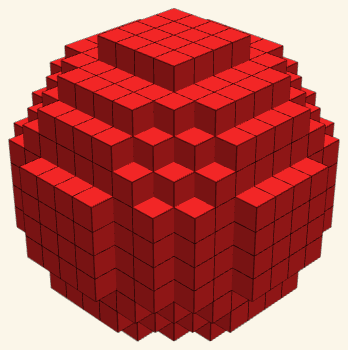
\includegraphics[width=0.55\linewidth]{fig07_3d_sphere_d12.png}\\[0.6em]
    {\sffamily\footnotesize\color{muted}Esfera de diâmetro 12 voxelizada pelo Pixel Round.}
  \end{minipage}
  \vspace{1.0cm}\\
  {\color{rule}\rule{0.6\textwidth}{0.6pt}\par}
  \vspace{1.0cm}
  \begin{minipage}{0.82\textwidth}
    \centering\sffamily\small\color{muted}
    \textbf{Áreas integradas:} Matemática $\cdot$ Linguagens (Arte digital, design) $\cdot$ Ciências da Natureza (ondas e luz) $\cdot$ Computação \\[0.4em]
    \textbf{Alinhamento:} BNCC --- Ensino Médio $\cdot$ Novo Ensino Médio (Lei 14.945/2024) $\cdot$ ENEM $\cdot$ \hyperref[sec:obmep]{OBMEP}
  \end{minipage}
\end{titlepage}

% =============================================================================
% SUMARIO
% =============================================================================
\renewcommand{\contentsname}{\color{accent}Sumário}
\tableofcontents
\thispagestyle{fancy}
\newpage

% =============================================================================
\section{Identificação e contextualização}\label{sec:identificacao}

\begin{center}
\begin{tabular}{@{}p{0.32\textwidth}p{0.62\textwidth}@{}}
\toprule
\textbf{Componente curricular} & Matemática (com articulação interdisciplinar). \\
\addlinespace[2pt]
\textbf{Etapa e ano} & Ensino Médio --- 3.\textordmasculine\ ano. Adaptável para 2.\textordmasculine\ ano e para a Educação de Jovens e Adultos (EJA). \\
\addlinespace[2pt]
\textbf{Modalidades atendidas} & Regular diurno, regular noturno, EJA, ensino integral, ensino técnico (cursos integrados ao EM nos Institutos Federais e CEFETs). \\
\addlinespace[2pt]
\textbf{Carga horária} & 4 aulas de 50 minutos (200 min em sala) + atividades extraclasse opcionais. Variante de 2 aulas geminadas de 100 min descrita em §\ref{sec:adapt}. \\
\addlinespace[2pt]
\textbf{Recurso central} & Pixel Round --- aplicação \emph{web} gratuita, sem cadastro, sem servidor, executa offline no navegador (PWA). Conforme a LGPD: não coleta nem transmite dados pessoais. \\
\addlinespace[2pt]
\textbf{Eixos BNCC} & Geometria e Medidas $\cdot$ Números e Álgebra $\cdot$ TCT \emph{Cultura Digital} (Tema Contemporâneo Transversal). \\
\addlinespace[2pt]
\textbf{Itinerários formativos (NEM)} & \emph{Matemática e suas Tecnologias} (principal); \emph{Ciências da Natureza e suas Tecnologias} (acústica); \emph{Linguagens e suas Tecnologias} (arte digital). Adequado a unidades curriculares de Aprofundamento e a projetos de Vida e Iniciação Científica. \\
\addlinespace[2pt]
\textbf{Articulações} & \hyperref[sec:obmep]{OBMEP} (Olimpíada Brasileira de Matemática das Escolas Públicas) $\cdot$ OBI (Olimpíada Brasileira de Informática) $\cdot$ Feiras de Ciências escolares e regionais. \\
\addlinespace[2pt]
\textbf{Conhecimentos prévios do aluno} & Plano cartesiano; equação da circunferência (1.\textordmasculine\ ano); área e volume de figuras elementares (2.\textordmasculine\ ano); noção de função; proporção e porcentagem. \\
\addlinespace[2pt]
\textbf{Preparo do professor} & 15 minutos de exploração prévia do Pixel Round; leitura de \texttt{docs\_math/Pixel\_Round\_Math\_pt-BR.pdf} (documento técnico em português). \\
\bottomrule
\end{tabular}
\end{center}

\begin{nota}[Diversidade da escola pública brasileira]
Esta sequência foi pensada para o contexto plural do Ensino Médio público brasileiro: a escola estadual urbana de São Paulo, Recife ou Manaus; o Instituto Federal num município do interior; o CEFET; a escola do campo em assentamento de reforma agrária; a escola indígena em terra demarcada; a escola quilombola; a EJA no turno noturno; o programa Pé-de-Meia (Lei 14.818/2024). Cada um desses contextos pede ajustes específicos, mapeados em §\ref{sec:adapt}. O Pixel Round foi escolhido porque \emph{atende todos eles}: roda em smartphone de baixo custo, dispensa internet após a primeira carga (PWA), não exige cadastro nem CPF, e não coleta dados pessoais --- condição exigida pela LGPD.
\end{nota}

% =============================================================================
\section{Justificativa pedagógica}\label{sec:justificativa}

A escolha do Pixel Round como artefato didático para o 3.\textordmasculine\ ano do Ensino Médio responde a uma demanda \acc{quádrupla} da educação brasileira contemporânea: integrar matemática formal e cultura digital (competência geral 5 da BNCC); contextualizar o conhecimento abstrato em práticas significativas para o estudante; preparar para itens de Geometria Espacial e Funções recorrentes no ENEM; e dialogar com o Novo Ensino Médio (Lei 14.945/2024) no eixo \emph{Matemática e suas Tecnologias}, em especial nos itinerários formativos de Aprofundamento.

O \emph{pixel art} ocupa lugar relevante no imaginário juvenil contemporâneo --- presente nos jogos eletrônicos (de Minecraft à produção independente brasileira como \emph{Dandara}, da Long Hat House em Belo Horizonte, ou \emph{Horizon Chase}, da Aquiris Game Studio em São Paulo), nas redes sociais e em produções audiovisuais. Tomá-lo como ponto de partida transforma uma tradição visual familiar em \emph{problema matemático genuíno}: descrever, em uma grade discreta, formas analiticamente definidas sobre $\mathbb{R}$.

Esse movimento didático opera em diálogo com cinco tradições da pedagogia brasileira:

\begin{itemize}[leftmargin=1.3em,itemsep=0.2em,topsep=0.3em]
  \item \acc{Paulo Freire} (\emph{Pedagogia do Oprimido}, 1968; \emph{Pedagogia da Autonomia}, 1996). O ponto de partida é a cultura visual concreta do estudante --- e não a abstração da equação --- o que aproxima a sequência da noção freireana de \emph{tema gerador}, evitando a \emph{educação bancária}. A construção coletiva do conceito de ``critério de pertinência'' realiza o que Freire chamou de \emph{problematização}.

  \item \acc{Ubiratan D'Ambrosio} (\emph{Etnomatemática}, 1985 em diante; ICMI Felix Klein Award, 2005). Diferentes culturas constroem diferentes ``modos de fazer'' matemática. Os três algoritmos do Pixel Round (Euclidiano, Bresenham, Limiar) podem ser lidos como três etnomatemáticas distintas para o mesmo problema --- recurso poderoso para a escola pública brasileira, onde a diversidade cultural é constitutiva.

  \item \acc{Anísio Teixeira} (Escola Nova brasileira; fundador do INEP). A defesa da escola pública gratuita, universal e laica, e o princípio de que aprende-se fazendo (\emph{learning by doing}) estruturam todas as atividades práticas da sequência.

  \item \acc{Darcy Ribeiro} (\emph{Sobre o óbvio}, 1986; idealizador dos CIEPs). A integração entre arte, ciência e técnica no mesmo espaço escolar inspira a articulação interdisciplinar da Aula~\ref{aula4}.

  \item \acc{Modelagem Matemática} brasileira (Bassanezi, Burak, Almeida, Caldeira). O Pixel Round materializa o ciclo clássico da modelagem: situação real $\rightarrow$ modelo matemático $\rightarrow$ análise computacional $\rightarrow$ confronto com a realidade $\rightarrow$ refinamento.
\end{itemize}

A presença do software cumpre função epistêmica precisa: \emph{não substitui} a álgebra, mas \emph{materializa} a diferença entre formulações matemáticas concorrentes. Os três algoritmos correspondem a três definições matematicamente distintas do mesmo objeto --- a circunferência discreta --- e produzem desenhos visivelmente diferentes, como ilustra a Figura~\ref{fig:comp-d10}. O aluno percebe, pelos olhos, que \emph{a definição importa}.

\begin{figure}[H]
\centering
\begin{subfigure}[t]{0.31\linewidth}\centering
  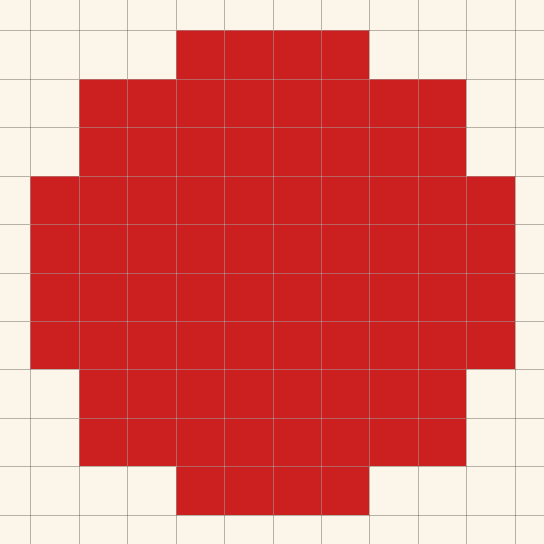
\includegraphics[width=\linewidth]{fig16_2d_d10_euclidean.png}
  \caption{\emph{Euclidiano}}
\end{subfigure}\hfill
\begin{subfigure}[t]{0.31\linewidth}\centering
  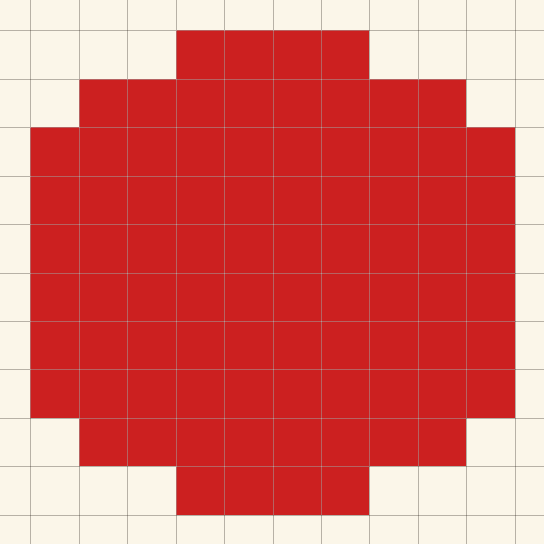
\includegraphics[width=\linewidth]{fig15_2d_d10_bresenham.png}
  \caption{\emph{Bresenham}}
\end{subfigure}\hfill
\begin{subfigure}[t]{0.31\linewidth}\centering
  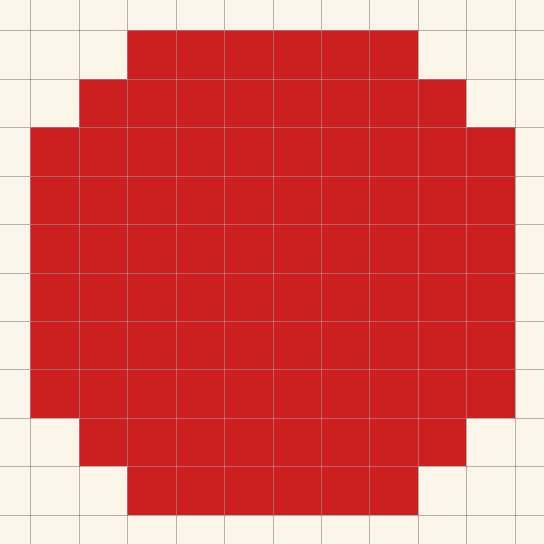
\includegraphics[width=\linewidth]{fig17_2d_d10_threshold.png}
  \caption{\emph{Limiar}}
\end{subfigure}
\caption{Mesma circunferência de diâmetro 10 sob três critérios de pertinência. Observe como a célula de canto, a transição entre linhas e os pontos cardeais variam de uma para outra --- são três respostas \emph{matematicamente corretas} sob critérios distintos.}
\label{fig:comp-d10}
\end{figure}

\begin{nota}[Equidade e a realidade material da escola pública]
A escolha do Pixel Round responde, em parte, a um problema material concreto: a desigualdade de acesso a recursos digitais entre escolas públicas brasileiras. O Censo Escolar do INEP (2023) registra que somente 65\% das escolas públicas de Ensino Médio possuem laboratório de informática em funcionamento, com variação regional acentuada. Por outro lado, o índice de posse de \emph{smartphones} pelos próprios estudantes é alto em todas as regiões (PNAD Contínua TIC 2023 indica mais de 90\% entre jovens de 15--17 anos). O Pixel Round foi projetado para funcionar exatamente nesse cenário: smartphone de baixo custo, sem internet permanente, sem cadastro --- e, quando necessário, o Apêndice~\ref{ap:adapt-analog} oferece um itinerário \emph{totalmente analógico} para uso exclusivo de papel quadriculado.
\end{nota}

% =============================================================================
\section{Objetivos}\label{sec:objetivos}

\subsection{Objetivo geral}

Conduzir os estudantes a \acc{compreender, comparar e utilizar} as definições formais da circunferência, da elipse e do elipsóide como critérios de inclusão de células em uma malha discreta, mobilizando a equação implícita dessas figuras para explicar, prever e modificar produções visuais autorais em \emph{pixel art} e \emph{voxel art}, em diálogo com o patrimônio cultural visual brasileiro (modernismo, arte concreta, grafismo dos povos originários) e com a tradição matemática nacional. A consciência dessa multiplicidade de respostas válidas conecta-se a uma cultura matemática brasileira que, em 2014, viu \hyperref[sec:obmep]{Artur Avila} tornar-se o primeiro latino-americano a receber a Medalha Fields.

\subsection{Objetivos específicos}

\textbf{Cognitivos (conceituais):}
\begin{itemize}[leftmargin=1.3em,itemsep=0.2em,topsep=0.3em]
  \item identificar a equação implícita $\left(\dfrac{x}{r_x}\right)^{\!2} + \left(\dfrac{y}{r_y}\right)^{\!2} = 1$ como caso geral que contém a circunferência $x^2 + y^2 = r^2$;
  \item reconhecer que três critérios distintos de pertinência (distância no centro, ponto médio de Bresenham, cobertura de quina) produzem três conjuntos diferentes de células --- como já visto na Figura~\ref{fig:comp-d10};
  \item compreender a transição da equação 2D para a equação 3D do elipsóide e relacioná-la com o cálculo de volume $V = \tfrac{4}{3}\pi r_x r_y r_z$ (assunto recorrente no ENEM, eixo \emph{Geometria});
  \item interpretar o corte de um sólido por um plano como uma \emph{desigualdade linear} aplicada às coordenadas dos voxels.
\end{itemize}

\textbf{Procedimentais:}
\begin{itemize}[leftmargin=1.3em,itemsep=0.2em,topsep=0.3em]
  \item operar a interface do Pixel Round em ambos os modos (2D e 3D) e exportar imagens em PNG;
  \item desenhar manualmente, em papel quadriculado, a aproximação discreta de uma circunferência aplicando o critério euclidiano e verificá-la no software;
  \item calcular a área discreta de uma elipse contando células e comparar com a área contínua $\pi r_x r_y$, expressando o resultado como erro relativo;
  \item compor uma figura autoral combinando círculos, elipses e elipsóides com justificativa matemática das escolhas.
\end{itemize}

\textbf{Atitudinais:}
\begin{itemize}[leftmargin=1.3em,itemsep=0.2em,topsep=0.3em]
  \item cooperar em duplas ou trios na produção das atividades práticas;
  \item argumentar matematicamente em defesa de uma escolha estética --- competência diretamente cobrada na redação do ENEM e em discussões orais de iniciação científica;
  \item reconhecer que problemas reais admitem mais de uma resposta tecnicamente correta;
  \item identificar referências matemáticas no patrimônio cultural brasileiro e nos saberes ancestrais.
\end{itemize}

% =============================================================================
\section{Competências e habilidades da BNCC}\label{sec:bncc}

A sequência mobiliza diretamente \acc{quatro habilidades} da área de Matemática e suas Tecnologias do Ensino Médio, além de articular-se com o Tema Contemporâneo Transversal \emph{Cultura Digital} e com habilidades de Linguagens e Ciências da Natureza.

\begin{habilidade}[EM13MAT307]
Empregar diferentes métodos para a obtenção da medida da área de uma superfície (reconfigurações, aproximação por cortes etc.) e \acc{deduzir expressões} de cálculo para aplicá-las em situações reais, \emph{com ou sem apoio de tecnologias digitais}.
\end{habilidade}

\begin{habilidade}[EM13MAT309]
Resolver e elaborar problemas que envolvem o \acc{cálculo de áreas totais e de volumes} de prismas, pirâmides e \emph{corpos redondos} em situações reais, \emph{com ou sem apoio de tecnologias digitais}.
\end{habilidade}

\begin{habilidade}[EM13MAT308]
Aplicar as relações métricas, incluindo as leis do seno e do cosseno ou as noções de congruência e semelhança, para resolver e elaborar problemas que envolvem triângulos em variados contextos.
\end{habilidade}

\begin{habilidade}[EM13MAT404]
Analisar funções definidas por uma ou mais sentenças, em suas representações algébrica e gráfica, identificando domínios de validade, imagem, crescimento e decrescimento, \acc{convertendo essas representações de uma para outra}, com ou sem apoio de tecnologias digitais.
\end{habilidade}

\medskip
Mobilizam-se ainda as \emph{competências específicas} de Matemática:

\begin{itemize}[leftmargin=1.3em,itemsep=0.15em,topsep=0.3em]
  \item \acc{Competência 3} --- construir modelos para resolver problemas, analisando a plausibilidade dos resultados;
  \item \acc{Competência 4} --- utilizar com flexibilidade diferentes registros de representação matemáticos (algébrico, geométrico, computacional);
  \item \acc{Competência 5} --- investigar e estabelecer conjecturas empregando estratégias e tecnologias diversas.
\end{itemize}

\subsection{Articulação com o ENEM}\label{sec:enem}

As habilidades acima conectam-se com os seguintes \emph{descritores} da Matriz de Referência do ENEM:

\begin{itemize}[leftmargin=1.3em,itemsep=0.15em,topsep=0.3em]
  \item Competência de Área 2 (\emph{Utilizar o conhecimento geométrico para realizar a leitura e a representação da realidade}), com destaque para H7 (geometria plana), H8 (medidas) e H9 (volumes e áreas);
  \item Competência de Área 3 (\emph{Construir noções de variação de grandezas para a compreensão da realidade e a solução de problemas do cotidiano}), descritor H12;
  \item Competência de Área 5 (\emph{Modelar e resolver problemas que envolvem variáveis socioeconômicas ou técnico-científicas, usando representações algébricas}), descritor H21.
\end{itemize}

A matriz oficial pode ser consultada no portal do \href{https://www.gov.br/inep/}{INEP}, na seção \emph{Avaliação e Exames Educacionais} $\rightarrow$ \emph{ENEM}.

\subsection{Tema Contemporâneo Transversal}

O TCT \acc{Cultura Digital} atravessa toda a sequência. Discutem-se questões de \emph{ética digital} (licenças de software livre \emph{vs.} proprietário), \emph{proteção de dados pessoais} (\href{https://www.planalto.gov.br/ccivil_03/_ato2015-2018/2018/lei/l13709.htm}{LGPD, Lei 13.709/2018}), e \emph{produção autoral} (direitos sobre as criações dos estudantes na Aula~\ref{aula4}).

% =============================================================================
\section{Conteúdos}\label{sec:conteudos}

\subsection{Conceituais}
\begin{itemize}[leftmargin=1.3em,itemsep=0.15em,topsep=0.3em]
  \item Plano cartesiano e sistema de coordenadas em $\mathbb{R}^2$ e $\mathbb{R}^3$; centro de uma célula \emph{vs.} canto.
  \item Equação reduzida da circunferência: $x^2 + y^2 = r^2$.
  \item Equação implícita geral da elipse: $\left(\dfrac{x}{r_x}\right)^{\!2} + \left(\dfrac{y}{r_y}\right)^{\!2} = 1$.
  \item Desigualdade da pertinência: \emph{interior, exterior} e \emph{fronteira}.
  \item Equação do elipsóide e da esfera em $\mathbb{R}^3$.
  \item Volume contínuo do elipsóide: $V = \tfrac{4}{3}\pi r_x r_y r_z$.
  \item Planos no espaço como desigualdades lineares (operação de corte).
  \item Vizinhança de uma célula (4-conectada em 2D, 6-conectada em 3D).
\end{itemize}

\subsection{Procedimentais}
\begin{itemize}[leftmargin=1.3em,itemsep=0.15em,topsep=0.3em]
  \item Traçado manual em papel quadriculado seguindo um critério explícito.
  \item Operação do Pixel Round (mudança de modo, ajuste de \emph{sliders}, escolha de algoritmo, exportação como PNG).
  \item Comparação de áreas discreta e contínua por contagem.
  \item Composição de figuras combinadas (\emph{pixel art} autoral com fundamentação geométrica).
\end{itemize}

\subsection{Atitudinais}
\begin{itemize}[leftmargin=1.3em,itemsep=0.15em,topsep=0.3em]
  \item Trabalho cooperativo em duplas ou trios.
  \item Argumentação fundamentada (justificar escolhas com matemática).
  \item Ética digital: respeito à licença do software e às produções dos colegas.
  \item Valorização de referências matemáticas presentes em saberes brasileiros.
\end{itemize}

\subsection{Modos de renderização e variedade de algoritmos}

Além de mudar o algoritmo, o Pixel Round oferece três \emph{modos de renderização} (Preenchido, Fino, Grosso) que produzem visuais distintos para a mesma figura geométrica, como ilustra a Figura~\ref{fig:render-modes}.

\begin{figure}[H]
\centering
\begin{subfigure}[t]{0.31\linewidth}\centering
  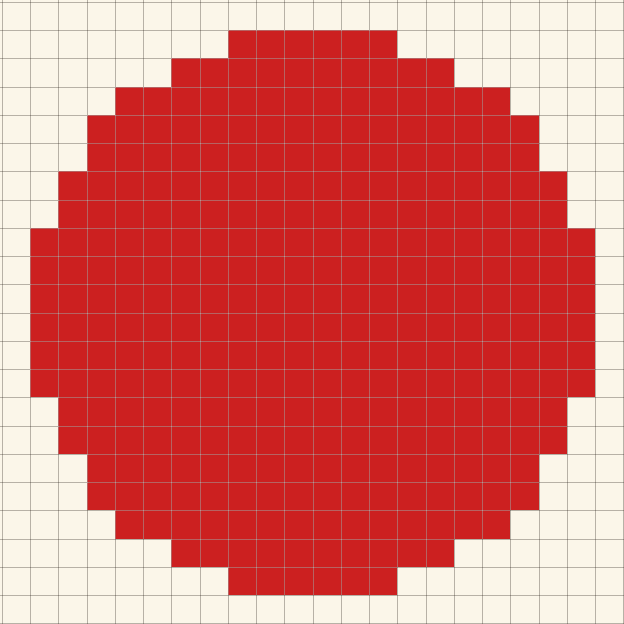
\includegraphics[width=\linewidth]{fig01_2d_d20_euclidean.png}
  \caption{\emph{Preenchido}}
\end{subfigure}\hfill
\begin{subfigure}[t]{0.31\linewidth}\centering
  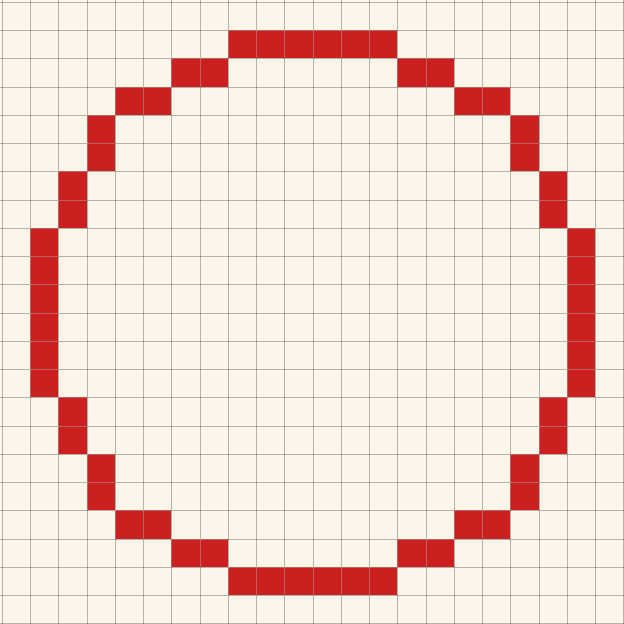
\includegraphics[width=\linewidth]{fig05_2d_d20_thin.png}
  \caption{\emph{Fino} (contorno de 1 px)}
\end{subfigure}\hfill
\begin{subfigure}[t]{0.31\linewidth}\centering
  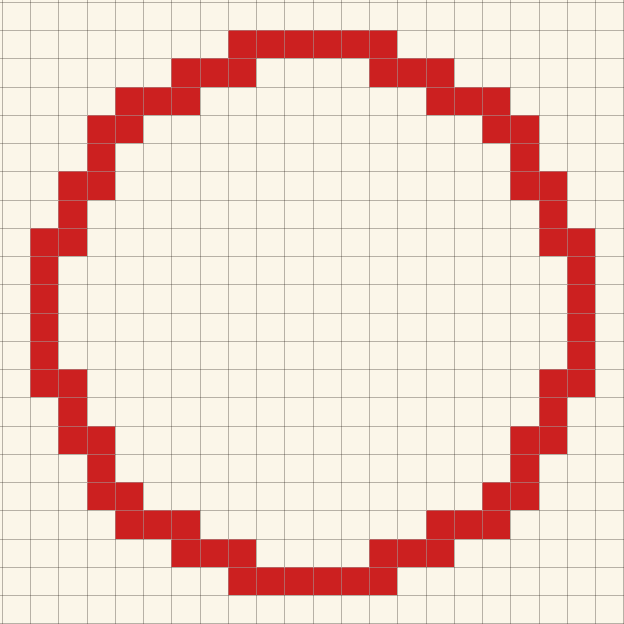
\includegraphics[width=\linewidth]{fig06_2d_d20_thick.png}
  \caption{\emph{Grosso} (contorno com pontes diagonais)}
\end{subfigure}
\caption{Os três modos de renderização para a mesma circunferência euclidiana de diâmetro 20. O modo \emph{Fino} corresponde ao bordo discreto topológico; o modo \emph{Grosso} adiciona pixels nas diagonais para evitar buracos a $45^\circ$.}
\label{fig:render-modes}
\end{figure}

% =============================================================================
\section{Conhecimentos prévios}\label{sec:prerrequisitos}

A sequência pressupõe contato anterior com:

\begin{itemize}[leftmargin=1.3em,itemsep=0.15em,topsep=0.3em]
  \item Plano cartesiano: localização de pontos $(x, y)$ e $(x, y, z)$.
  \item Equação reduzida da circunferência (conteúdo de 1.\textordmasculine\ ano EM).
  \item Áreas de polígonos e do círculo; volumes de cubo, prisma e cilindro (conteúdo de 2.\textordmasculine\ ano EM).
  \item Conceito de função: domínio, imagem, gráfico.
  \item Noção de proporção e porcentagem.
\end{itemize}

Caso a turma demonstre defasagem em algum desses pontos --- realidade frequente no contexto pós-pandemia, conforme dados do \href{https://www.gov.br/inep/pt-br/areas-de-atuacao/avaliacao-e-exames-educacionais/saeb}{SAEB} 2023 que mostram queda nos indicadores de Matemática em diversas redes ---, a \emph{Aula 1} dispõe de um momento de \emph{nivelamento diagnóstico} (10 min) descrito em §\ref{aula1}.

% =============================================================================
\section{Recursos e materiais}\label{sec:recursos}

\subsection{Recursos digitais}
\begin{itemize}[leftmargin=1.3em,itemsep=0.15em,topsep=0.3em]
  \item Pixel Round (uma instância por estudante \emph{ou} por dupla);
  \item Projetor multimídia, TV com entrada HDMI ou lousa digital interativa;
  \item Acesso a \emph{laboratório de informática} \emph{ou} uso de \emph{smartphones} pessoais (BYOD --- \emph{Bring Your Own Device}) \emph{ou} \emph{tablets} distribuídos por programas estaduais.
\end{itemize}

\subsection{Recursos analógicos}
\begin{itemize}[leftmargin=1.3em,itemsep=0.15em,topsep=0.3em]
  \item Papel quadriculado (1\,cm), 2 folhas por estudante;
  \item Lápis preto, borracha, régua de 30\,cm;
  \item Lápis de cor ou canetinhas (preferencialmente vermelho \texttt{\#CC2020} e preto);
  \item Folha de exercícios (Apêndice~\ref{ap:exerc});
  \item Lousa convencional ou quadro branco.
\end{itemize}

\subsection{Livro didático e PNLD}\label{sec:pnld}

O Pixel Round complementa --- não substitui --- o livro didático adotado pela escola via \href{https://www.gov.br/fnde/pt-br/acesso-a-informacao/acoes-e-programas/programas/programas-do-livro}{PNLD} (Programa Nacional do Livro e do Material Didático). Coleções recomendadas que cobrem os conteúdos mobilizados:

\begin{itemize}[leftmargin=1.3em,itemsep=0.1em,topsep=0.2em,nosep]
  \item \emph{Matemática Contexto e Aplicações} (Luiz Roberto Dante), Ática;
  \item \emph{Matemática: Ciência e Aplicações} (Iezzi, Dolce, Degenszajn, Périgo, Almeida), Saraiva;
  \item \emph{Matemática Paiva} (Manoel Paiva), Moderna;
  \item \emph{Conexões com a Matemática} (Fábio Martins de Leonardo \emph{et al.}), Moderna.
\end{itemize}

Os capítulos sobre \emph{equação da circunferência}, \emph{cônicas} e \emph{geometria espacial métrica} (volumes) dialogam diretamente com a sequência.

\subsection{Acesso ao Pixel Round}

Em ordem de preferência:

\begin{enumerate}[leftmargin=1.5em,itemsep=0.15em,topsep=0.3em]
  \item \textbf{Hospedado pelo professor} em \emph{GitHub Pages} ou no portal da escola (URL distribuída por QR Code projetado na lousa).
  \item \textbf{Cópia local} dos arquivos do projeto em uma pasta do laboratório, executada via \emph{file://}.
  \item \textbf{Offline em \emph{smartphone}} via PWA: basta abrir uma vez com internet para que o navegador instale o aplicativo.
\end{enumerate}

% =============================================================================
\section{Adaptações para a realidade plural brasileira}\label{sec:adapt}

A escola pública brasileira é heterogênea --- talvez a mais heterogênea do mundo entre redes nacionais. Esta sequência foi desenhada para se adaptar a essa pluralidade, com variantes específicas para cada contexto.

\subsection{Escolas estaduais urbanas (capital ou região metropolitana)}
Cenário típico de São Paulo, Belo Horizonte, Salvador, Fortaleza. Geralmente dispõe de laboratório de informática (uso compartilhado), lousa digital e Wi-Fi razoável. \emph{Configuração mais simples para implementar a sequência integralmente em laboratório.}

\subsection{Escolas estaduais urbanas (interior)}
Realidade da grande maioria dos municípios brasileiros. Laboratório de informática pode estar parcialmente operacional. Recomenda-se \emph{modelo BYOD} com \emph{smartphones} pessoais dos estudantes, organizados em duplas (um celular por dupla). É a configuração \acc{mais comum} no país.

\subsection{Institutos Federais (IFs) e CEFETs}
Rede federal de excelência técnica. Geralmente bem equipada. A sequência integra-se naturalmente aos cursos técnicos integrados ao Ensino Médio (Informática, Eletrônica, Design Gráfico, Multimídia). Recomenda-se aprofundar a Aula~\ref{aula2} (algoritmo de Bresenham) com implementação em Python no laboratório.

\subsection{Escolas do campo}
Cenário do PRONERA (Programa Nacional de Educação na Reforma Agrária) e da Educação do Campo. Tradicionalmente menos equipadas digitalmente, mas com \emph{forte conhecimento prévio geométrico} dos estudantes (geometria aplicada a roçados, cercas, irrigação). Recomenda-se variante analógica (Apêndice~\ref{ap:adapt-analog}) e dispositivo único do professor para demonstração.

\subsection{Escolas indígenas e quilombolas}
A \href{https://www.planalto.gov.br/ccivil_03/_ato2007-2010/2008/lei/l11645.htm}{Lei 11.645/2008} estabelece a obrigatoriedade do ensino de história e cultura afro-brasileira e indígena. Esta sequência pode ser \emph{enriquecida com saberes próprios da comunidade}: o grafismo Kadiwéu (MS), as cestarias trançadas dos povos Wayuu, Kayapó e Yanomami, a cerâmica marajoara (PA) ou a estatuária Karajá. \emph{O professor de Arte e os anciãos da comunidade são parceiros essenciais nessa adaptação} (ver Aula~\ref{aula3}, Atividade~\ref{at:34}).

\subsection{Educação de Jovens e Adultos (EJA)}
Tipicamente turmas noturnas, com estudantes adultos que retornam à escola. O Pixel Round funciona bem aqui porque a interface é amigável e o tema (pixel art / videogames) é também familiar a essa faixa etária. Sugere-se reduzir o tempo de cada atividade em 20\% (em virtude do turno mais curto da EJA) e priorizar discussões orais em vez de produção escrita longa.

\subsection{Variante para 2 aulas geminadas (100 min cada)}
Para escolas com horário em \emph{módulo duplo} (frequente em IFs e em projetos de tempo integral): Aulas 1+2 num módulo, 3+4 no outro, com 10 min de intervalo no meio de cada módulo.

\subsection{Crosswalk com Currículos Referenciais Estaduais}

Cada secretaria estadual de educação detalhou a BNCC em seu próprio currículo referencial. As principais redes:

\begin{center}
\small
\begin{tabularx}{\textwidth}{@{}p{0.18\textwidth}p{0.25\textwidth}X@{}}
\toprule
\textbf{Rede} & \textbf{Currículo de referência} & \textbf{Habilidades equivalentes a EM13MAT307/309} \\
\midrule
SEDUC-SP & Currículo Paulista (2020) & Bimestre de Geometria, 3.\textordmasculine\ EM, eixo \emph{Geometria e Medidas}. \\
\addlinespace[3pt]
SEEDUC-RJ & Currículo Mínimo Estadual & Unidade temática \emph{Geometria espacial métrica}. \\
\addlinespace[3pt]
SEE-MG & Currículo Referência de MG & Eixo \emph{Geometria}, 3.\textordmasculine\ EM. \\
\addlinespace[3pt]
SEDUC-CE & DCRC (Documento Curricular Referencial do Ceará) & Geometria espacial métrica e analítica. \\
\addlinespace[3pt]
SEDUC-AM & Currículo Referência do Amazonas & Geometria com itinerário integrado a \emph{Aprofundamento em STEM}. \\
\bottomrule
\end{tabularx}
\end{center}

\subsection{Ensino híbrido ou remoto}
A natureza \emph{web} do Pixel Round o torna trivialmente compatível com aulas remotas (\emph{Google Meet}, \emph{Zoom}, plataformas estaduais como \emph{CMSP} de São Paulo ou \emph{Sala de Aula Digital} de outras redes). O professor compartilha sua tela; estudantes acompanham na própria máquina. As atividades em papel quadriculado podem ser fotografadas e enviadas como tarefa assíncrona via WhatsApp do grupo da turma, Google Classroom ou plataforma da rede.

% =============================================================================
\section{Sequência didática}\label{sec:sequencia}

A sequência segue a estrutura \acc{mobilização --- problematização --- sistematização --- síntese}, inspirada nos \emph{três momentos pedagógicos} de Delizoicov \& Angotti (1990) e na tradição freireana de partir do conhecimento prévio do estudante. Cada aula de 50 minutos respeita o ritmo cognitivo do adolescente, alternando momentos expositivos breves ($\leq 15$\,min) com atividades práticas.

% =============================================================================
\subsection{Aula 1 --- ``Como o computador desenha um círculo com quadradinhos?''}\label{aula1}

\subsubsection*{Objetivo da aula}
Estabelecer o \emph{problema central} da rasterização discreta como um problema matemático genuíno, mobilizar a equação da circunferência e apresentar o Pixel Round.

\begin{atividade}[1.1 --- Mobilização \quad\tempo{10 min}]
\textbf{Estratégia:} \emph{think--pair--share} (pensar individualmente, conversar em dupla, compartilhar com a turma). \\[0.4em]
\textbf{Passo a passo:}
\begin{enumerate}[leftmargin=1.5em,itemsep=0.2em,topsep=0.3em,nosep]
  \item Projetar (ou desenhar) três \emph{sprites} clássicos de \emph{pixel art}: o cogumelo de \emph{Super Mario} (Nintendo, marco do gênero), um Pokémon de primeira geração e um personagem de jogo brasileiro \emph{pixel art}, como \emph{Dandara} (Long Hat House, BH) ou \emph{Horizon Chase} (Aquiris, SP).
  \item Perguntar à turma: \emph{``Olhem com atenção. O que esses três desenhos têm em comum? O que diferencia o desenho dos jogos do desenho de um círculo feito com compasso na aula passada?''}
  \item Cada estudante anota individualmente sua resposta (1\,min) e em seguida discute com o colega ao lado (2\,min).
  \item Recolha coletiva: anotar respostas-chave no canto da lousa. Conduzir para a observação fundamental: \emph{``o computador só consegue acender quadradinhos --- como ele decide quais?''}
\end{enumerate}
\end{atividade}

\begin{atividade}[1.2 --- Problematização \quad\tempo{15 min}]
\textbf{Estratégia:} desenho manual confrontado com a definição formal. \\[0.4em]
\textbf{Material:} papel quadriculado, lápis. \\[0.4em]
\textbf{Passo a passo:}
\begin{enumerate}[leftmargin=1.5em,itemsep=0.2em,topsep=0.3em,nosep]
  \item Cada estudante recebe meia folha de papel quadriculado e marca o ponto central de uma região $11 \times 11$ células.
  \item Comando: \emph{``Pintem o melhor círculo que vocês conseguirem com diâmetro 10 (raio 5). Vocês têm 4 minutos.''}
  \item Após o tempo, três ou quatro estudantes vão à lousa reproduzir seu desenho em uma malha desenhada com giz/marcador.
  \item Observação dirigida pelo professor: \emph{``Olhem. Vocês fizeram a mesma figura? Por quê não? Quem está certo?''}
  \item Sistematizar: não há \emph{uma única} resposta (a Figura~\ref{fig:comp-d10} apresentada na §\ref{sec:justificativa} corrobora). Cada estudante adotou implicitamente um \acc{critério} diferente para decidir se uma célula entra ou não.
\end{enumerate}

\textbf{Nota etnomatemática:} aproveitar o momento para mencionar que \emph{essa diversidade de respostas é exatamente o objeto da Etnomatemática} (Ubiratan D'Ambrosio), campo brasileiro reconhecido internacionalmente que estuda como diferentes culturas e grupos resolvem problemas matemáticos de maneiras distintas e igualmente válidas.
\end{atividade}

\begin{atividade}[1.3 --- Sistematização \quad\tempo{15 min}]
\textbf{Estratégia:} exposição dialogada com apoio do quadro. \\[0.4em]
\textbf{Conteúdo:}

A equação implícita da circunferência centrada na origem de raio $r$ é

\begin{formula}
\centering
$\displaystyle x^2 + y^2 \;=\; r^2$
\end{formula}

Pontos \emph{dentro} satisfazem $x^2 + y^2 < r^2$; pontos \emph{fora}, $x^2 + y^2 > r^2$. A equação se generaliza para a elipse de semi-eixos $r_x, r_y$:

\begin{formula}
\centering
$\displaystyle \left(\dfrac{x}{r_x}\right)^{\!2} + \left(\dfrac{y}{r_y}\right)^{\!2} \;=\; 1$
\end{formula}

Em uma malha de pixels, o desafio é decidir quais \acc{células} pertencem ao interior. Decisões diferentes geram desenhos diferentes. O Pixel Round implementa \emph{três} critérios:

\begin{itemize}[leftmargin=1.3em,itemsep=0.15em,topsep=0.3em]
  \item \acc{Euclidiano}: o centro $(i + \tfrac{1}{2},\, j + \tfrac{1}{2})$ da célula está dentro?
  \item \acc{Bresenham}: algoritmo histórico de 1965, opera apenas com inteiros.
  \item \acc{Limiar}: alguma \emph{quina} da célula está dentro?
\end{itemize}

\textbf{Demonstração:} o professor abre o Pixel Round, ajusta o diâmetro para 10, alterna entre os três algoritmos com a turma observando as diferenças. Sublinhar: as três figuras são \emph{matematicamente corretas} sob critérios distintos.
\end{atividade}

\begin{atividade}[1.4 --- Síntese \quad\tempo{10 min}]
\textbf{Estratégia:} aplicação imediata individual. \\[0.4em]
\textbf{Comando:} \emph{``Voltem ao papel. Refaçam o círculo de diâmetro 10 aplicando \acc{rigorosamente} o critério euclidiano: pintar a célula se, e somente se, o ponto central dela $(i + 0{,}5,\, j + 0{,}5)$ estiver a uma distância menor ou igual a 5 do centro.''}

Ao final, comparar o desenho do papel com o que o Pixel Round produz no algoritmo Euclidiano com diâmetro 10 --- a referência visual é a Figura~\ref{fig:comp-d10}~(a). \emph{Devem coincidir.}
\end{atividade}

\subsubsection*{Tarefa de casa (opcional)}
Repetir o exercício 1.4 com diâmetros 8 e 14. Trazer os três desenhos na aula seguinte.

% =============================================================================
\subsection{Aula 2 --- ``Três algoritmos, três desenhos''}\label{aula2}

\subsubsection*{Objetivo da aula}
Aprofundar a compreensão dos três algoritmos como definições matemáticas distintas e comparar quantitativamente os resultados.

\begin{atividade}[2.1 --- Retomada \quad\tempo{5 min}]
Recolher rapidamente os desenhos da tarefa de casa, observar variações na turma, anunciar o objetivo da aula: \emph{``Hoje vamos olhar para cada um dos três algoritmos com lupa, e descobrir por que Bresenham é considerado uma joia da Computação.''}
\end{atividade}

\begin{atividade}[2.2 --- Algoritmo Euclidiano \quad\tempo{10 min}]
Formalização. Para uma célula $(i, j)$, calcular as coordenadas normalizadas

\begin{formula}
\centering
$\displaystyle d_x = \dfrac{i + \tfrac{1}{2} - c_x}{r_x},\qquad d_y = \dfrac{j + \tfrac{1}{2} - c_y}{r_y}$
\end{formula}

A célula é pintada se, e somente se, $d_x^{\,2} + d_y^{\,2} \leq 1$.

\textbf{No quadro:} resolver explicitamente o caso $c_x = c_y = 5$, $r_x = r_y = 5$, célula $(2, 1)$. Tem-se $d_x = (2{,}5 - 5)/5 = -0{,}5$ e $d_y = (1{,}5 - 5)/5 = -0{,}7$, portanto $d_x^2 + d_y^2 = 0{,}25 + 0{,}49 = 0{,}74 \leq 1$. Célula \emph{dentro}. \\

Pedir aos estudantes que testem a célula $(0, 0)$ (qual o resultado?). Discutir.
\end{atividade}

\begin{atividade}[2.3 --- Algoritmo de Bresenham \quad\tempo{15 min}]\label{at:23}
\textbf{Contexto histórico:} Jack Bresenham publicou o algoritmo em 1965 quando trabalhava na IBM. Antes dele, traçar uma reta exigia operações em ponto flutuante --- caras nos computadores da época. Bresenham mostrou que era possível desenhar usando \emph{apenas inteiros}: somas e comparações.

A versão para circunferência usa um \emph{parâmetro de decisão} $d$. Começa-se em $(x{=}0,\, y{=}R)$ com $d_0 = 1 - R$. A cada passo no octante $0$--$45^\circ$:

\begin{formula}
\centering
$\begin{cases}
\text{se } d < 0: & \text{próximo: } (x{+}1,\, y),\; d \mathrel{+}= 2x+3 \\
\text{se } d \geq 0: & \text{próximo: } (x{+}1,\, y{-}1),\; d \mathrel{+}= 2(x-y)+5
\end{cases}$
\end{formula}

\textbf{Demonstração no quadro:} traçar passo a passo o algoritmo para $R = 5$, anotando $x, y, d$ a cada iteração. Os oito octantes são obtidos por simetria. \\

\textbf{Conexão com a OBI:} o algoritmo de Bresenham é tema clássico em provas da \href{https://olimpiada.ic.unicamp.br/}{Olimpíada Brasileira de Informática (OBI)}, organizada pela SBC (Sociedade Brasileira de Computação) na Unicamp. Estudantes interessados podem aprofundar via o material gratuito disponível no portal da OBI.

\textbf{Observação metodológica:} se a turma demonstrar dificuldade com a álgebra do parâmetro $d$, basta apresentar o algoritmo como uma \emph{regra} (sem demonstrar a função de decisão). A justificação completa está no documento técnico \texttt{Pixel\_Round\_Math\_pt-BR.pdf}, §5.
\end{atividade}

\begin{atividade}[2.4 --- Algoritmo de Limiar \quad\tempo{10 min}]
Para cada célula $(i, j)$, identificar a \emph{quina mais próxima} do centro da forma:

\begin{formula}
\centering
$\displaystyle n_x = \mathrm{clamp}(c_x,\, i,\, i{+}1),\qquad n_y = \mathrm{clamp}(c_y,\, j,\, j{+}1)$
\end{formula}

A célula é incluída se $\left(\dfrac{n_x - c_x}{r_x}\right)^{\!2} + \left(\dfrac{n_y - c_y}{r_y}\right)^{\!2} \leq 0{,}94$.

\textbf{Por que $0{,}94$ e não $1$?} Empiricamente, com $1$ aparecem ``espinhos'' de 1 pixel nos pontos cardeais. O limiar levemente menor elimina o artefato. \emph{Esta é uma decisão de engenharia tomada por inspeção visual} --- um exemplo importante de como a matemática teórica nem sempre basta sozinha. Em termos freireanos: a ``palavra final'' não é da fórmula, mas do diálogo entre teoria e prática.
\end{atividade}

\begin{atividade}[2.5 --- Comparação quantitativa \quad\tempo{10 min}]\label{at:25}
\textbf{Atividade prática em duplas.} No Pixel Round (ou no projetor centralizado):
\begin{enumerate}[leftmargin=1.5em,itemsep=0.15em,topsep=0.3em,nosep]
  \item Definir diâmetro 20 e modo \emph{Preenchido} (a Figura~\ref{fig:comp-d20} mostra o resultado esperado para cada algoritmo).
  \item Acionar o \emph{Info chip} no canto do canvas. Anotar a área de cada um dos três algoritmos.
  \item Calcular a área contínua: $\pi r^2 = \pi \cdot 10^2 \approx 314{,}16$.
  \item Para cada algoritmo, calcular o erro relativo: $\dfrac{|\text{área discreta} - \text{área contínua}|}{\text{área contínua}} \times 100\%$.
  \item Ordenar os três algoritmos do mais próximo ao mais distante do valor contínuo.
\end{enumerate}

\textbf{Resultado esperado:} Euclidiano costuma ficar muito próximo (erro abaixo de $2\%$); Limiar sobreestima em poucos por cento; Bresenham fica no meio. Confirmar coletivamente.
\end{atividade}

\begin{figure}[H]
\centering
\begin{subfigure}[t]{0.31\linewidth}\centering
  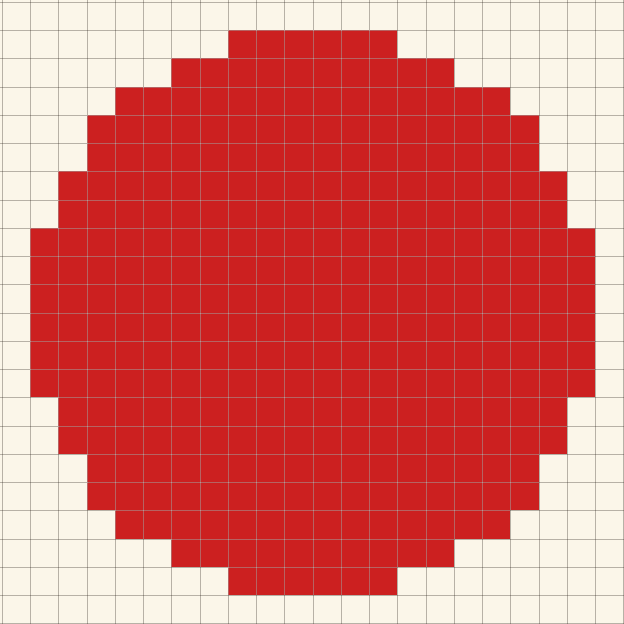
\includegraphics[width=\linewidth]{fig01_2d_d20_euclidean.png}
  \caption{\emph{Euclidiano}}
\end{subfigure}\hfill
\begin{subfigure}[t]{0.31\linewidth}\centering
  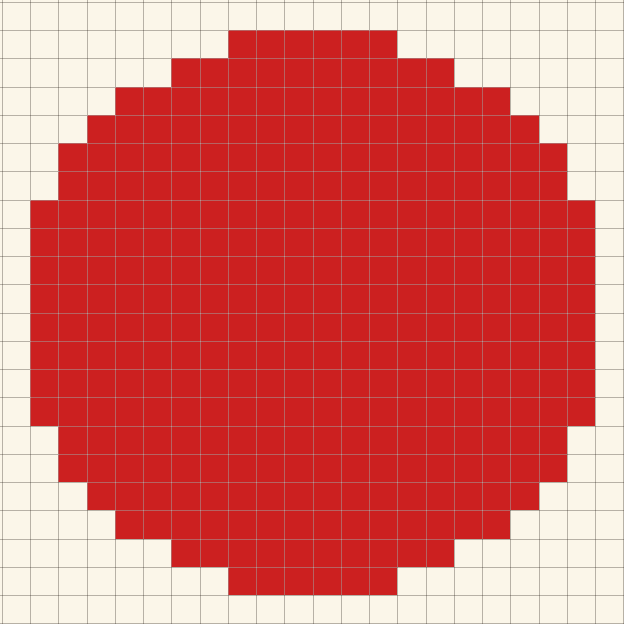
\includegraphics[width=\linewidth]{fig02_2d_d20_bresenham.png}
  \caption{\emph{Bresenham}}
\end{subfigure}\hfill
\begin{subfigure}[t]{0.31\linewidth}\centering
  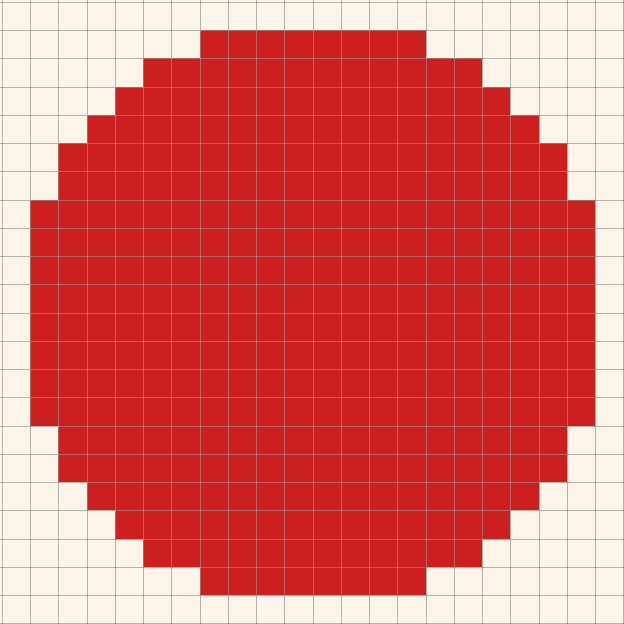
\includegraphics[width=\linewidth]{fig03_2d_d20_threshold.png}
  \caption{\emph{Limiar}}
\end{subfigure}
\caption{Mesma circunferência de diâmetro 20 nos três algoritmos. O aumento de diâmetro torna as diferenças mais sutis --- as três versões parecem semelhantes. É um bom momento para comentar que para diâmetros pequenos (Figura~\ref{fig:comp-d10}) as diferenças são muito mais evidentes.}
\label{fig:comp-d20}
\end{figure}

% =============================================================================
\subsection{Aula 3 --- ``Da elipse ao elipsóide: a terceira dimensão''}\label{aula3}

\subsubsection*{Objetivo da aula}
Generalizar a equação da elipse para o elipsóide, introduzir voxels, cálculo de volume discreto e cortes planares. Estabelecer pontes com a tradição visual brasileira.

\begin{atividade}[3.1 --- Da equação 2D para 3D \quad\tempo{15 min}]\label{at:31}
Acrescentar uma terceira coordenada $z$ ao plano cartesiano. A equação implícita da elipse generaliza-se naturalmente:

\begin{formula}
\centering
$\displaystyle \left(\dfrac{x}{r_x}\right)^{\!2} + \left(\dfrac{y}{r_y}\right)^{\!2} + \left(\dfrac{z}{r_z}\right)^{\!2} \;=\; 1$
\end{formula}

Quando $r_x = r_y = r_z = r$, recupera-se a \acc{esfera} $x^2 + y^2 + z^2 = r^2$, como ilustrado na Figura~\ref{fig:3d-shapes}.

\textbf{Voxels:} a célula de uma malha 3D chama-se \emph{voxel} (\emph{volume element}). O critério de pertinência é exatamente o mesmo do caso 2D, acrescido da coordenada $z$:

\begin{formula}
\centering
$\displaystyle a_x^2 + a_y^2 + a_z^2 \leq 1,\quad \text{com } a_\xi = \dfrac{\xi + \tfrac{1}{2} - c_\xi}{r_\xi}$
\end{formula}

\textbf{Demonstração:} abrir o Pixel Round no modo 3D, alternar entre Esfera e Elipsóide, rotacionar com o \emph{mouse}, observar a estrutura de voxels.
\end{atividade}

\begin{figure}[H]
\centering
\begin{subfigure}[t]{0.45\linewidth}\centering
  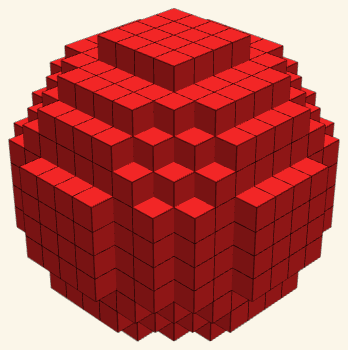
\includegraphics[width=\linewidth]{fig07_3d_sphere_d12.png}
  \caption{Esfera de diâmetro 12 ($r_x = r_y = r_z = 6$).}
\end{subfigure}\hfill
\begin{subfigure}[t]{0.45\linewidth}\centering
  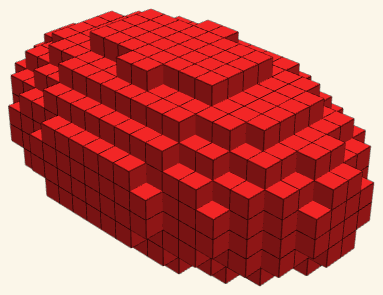
\includegraphics[width=\linewidth]{fig08_3d_ellipsoid.png}
  \caption{Elipsóide com $W = 20, H = 10, D = 12$.}
\end{subfigure}
\caption{Voxelização em 3D. Cada cubo é um voxel; sua coordenada $(i, j, k)$ no centro é testada na equação implícita.}
\label{fig:3d-shapes}
\end{figure}

\begin{atividade}[3.2 --- Volume contínuo \emph{vs.} discreto \quad\tempo{15 min}]\label{at:32}
O volume contínuo do elipsóide é um resultado clássico:

\begin{formula}
\centering
$\displaystyle V \;=\; \dfrac{4}{3}\,\pi\, r_x\, r_y\, r_z$
\end{formula}

Quando $r_x = r_y = r_z = r$, $V = \tfrac{4}{3}\pi r^3$. Este é um conteúdo \acc{recorrente no ENEM} (questões de Geometria Espacial cobradas em praticamente todas as edições) e também na fase 2 da \hyperref[sec:obmep]{OBMEP}, especialmente em problemas que envolvem aproximação numérica.

\textbf{Atividade em dupla:}
\begin{enumerate}[leftmargin=1.5em,itemsep=0.15em,topsep=0.3em,nosep]
  \item Calcular o volume contínuo de uma esfera de diâmetro 12 ($r = 6$): $V = \tfrac{4}{3}\pi \cdot 216 \approx 904{,}78$.
  \item No Pixel Round, gerar a esfera $D = 12$ (a mesma da Figura~\ref{fig:3d-shapes}(a)), modo \emph{Preenchido}, acionar \emph{Info chip}, anotar o volume discreto (número de voxels).
  \item Calcular o erro relativo, como na aula anterior.
\end{enumerate}

\textbf{Observação:} a relação $\text{volume discreto}/\text{volume contínuo} \to 1$ quando $D \to \infty$. Para $D$ pequeno, há divergência sensível --- e isso é matematicamente correto: a discretização \emph{de fato} altera a contagem.
\end{atividade}

\begin{atividade}[3.3 --- Cortes planares \quad\tempo{10 min}]\label{at:33}
O Pixel Round permite cortar o elipsóide por três planos diferentes. Cada corte é uma \acc{desigualdade linear} aplicada ao centro do voxel:

\begin{formula}
\centering
$\begin{array}{lcl}
\text{Eixo X:} & x \geq \mathit{cut} & \Rightarrow \text{voxel descartado} \\
\text{Eixo Y:} & y \geq \mathit{cut} & \Rightarrow \text{voxel descartado} \\
\text{Diagonal:} & x + y \geq \mathit{cut} & \Rightarrow \text{voxel descartado}
\end{array}$
\end{formula}

A Figura~\ref{fig:cortes} ilustra os três cortes a $50\%$.

\textbf{Discussão dirigida:} \emph{``Por que um corte diagonal tem amplitude $D_x + D_y$ e não $D_x$? Onde está a hipotenusa?''} Conduzir para o reconhecimento de que $x + y$ assume valores entre $0$ e $D_x + D_y$ na caixa retangular.
\end{atividade}

\begin{figure}[H]
\centering
\begin{subfigure}[t]{0.31\linewidth}\centering
  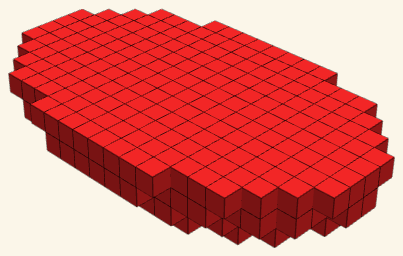
\includegraphics[width=\linewidth]{fig09_3d_cut_y50.png}
  \caption{Corte Y a 50\% ($y \geq 5$ descartado)}
\end{subfigure}\hfill
\begin{subfigure}[t]{0.31\linewidth}\centering
  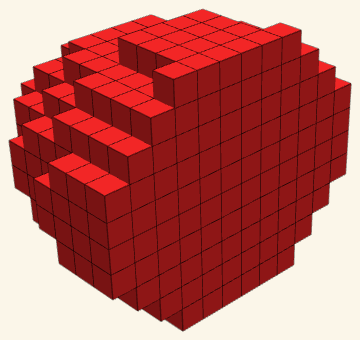
\includegraphics[width=\linewidth]{fig10_3d_cut_x50.png}
  \caption{Corte X a 50\% ($x \geq 10$ descartado)}
\end{subfigure}\hfill
\begin{subfigure}[t]{0.31\linewidth}\centering
  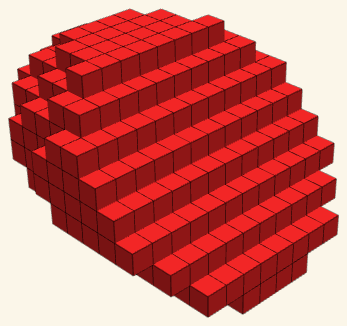
\includegraphics[width=\linewidth]{fig11_3d_cut_diag50.png}
  \caption{Corte diagonal ($x+y \geq 15$ descartado)}
\end{subfigure}
\caption{Três cortes planares no mesmo elipsóide ($W = 20, H = 10, D = 12$), todos preservando $50\%$ do volume. Observe o padrão escalonado característico do corte diagonal: ele expõe a hipotenusa que conecta os dois eixos.}
\label{fig:cortes}
\end{figure}

\begin{atividade}[3.4 --- Diálogo com o patrimônio visual brasileiro \quad\tempo{10 min}]\label{at:34}
\emph{Conexão com Linguagens e Arte. Esta atividade cumpre as competências da BNCC sobre identidade cultural e patrimônio.}

Projetar (ou distribuir impressas) três imagens:

\begin{itemize}[leftmargin=1.3em,itemsep=0.2em,topsep=0.3em,nosep]
  \item \acc{Catedral Metropolitana de Brasília} (Oscar Niemeyer, 1970): suas 16 colunas curvas constituem um \emph{hiperboloide de revolução} construído com concreto armado. Junto com o Palácio do Itamaraty, o Memorial JK e o MAC Niterói (este último abertamente elipsoidal, ver Figura~\ref{fig:3d-shapes}(b)), Niemeyer realizou em escala arquitetônica exatamente as quádricas que estamos estudando.

  \item \acc{Grafismo Kadiwéu} (MS): os desenhos corporais e em cerâmica do povo Kadiwéu, descritos por Claude Lévi-Strauss em \emph{Tristes Trópicos} (1955), são reconhecidos por sua sofisticação geométrica: \emph{simetrias dobradas}, partição do espaço em zonas circulares e quadrangulares justapostas. Tradição matemática viva, anterior à colonização.

  \item \acc{Cerâmica marajoara} (PA, séculos V--XIV): vasos e estatuetas com motivos circulares concêntricos, espirais e divisões geométricas. Patrimônio arqueológico brasileiro reconhecido pelo IPHAN.
\end{itemize}

\textbf{Discussão dirigida:} \emph{``Niemeyer projetou em concreto as mesmas curvas que vocês desenharam em pixels. Os povos Kadiwéu e marajoaras representaram círculos e simetrias usando barro, tinta corporal e tecido --- séculos antes dos computadores existirem. O problema da rasterização que estudamos não é uma invenção da era digital: é uma constante da história humana. Cada cultura encontrou seu modo de \emph{rasterizar}.''}

\textbf{Articulação interdisciplinar:} parceria sugerida com o(a) professor(a) de Arte e/ou de História para aprofundamento. A Aula~\ref{aula4} pode pedir que os grupos \emph{escolham} qual tradição visual brasileira inspirará seu trabalho.
\end{atividade}

% =============================================================================
\subsection{Aula 4 --- ``Projeto final: pixel art autoral com fundamentação matemática''}\label{aula4}

\subsubsection*{Objetivo da aula}
Mobilizar todo o conteúdo desenvolvido em um produto autoral, avaliando aprendizagem por meio da defesa argumentativa das escolhas matemáticas.

\begin{atividade}[4.1 --- Apresentação do desafio \quad\tempo{5 min}]\label{at:41}
\textbf{Comando:} \emph{``Em duplas ou trios, vocês vão produzir uma imagem de \emph{pixel art} ou \emph{voxel art} que combine, no mínimo, três figuras geradas pelo Pixel Round (círculos, elipses, esferas ou elipsóides). Pode ser um personagem, um ícone, um animal, um logo, uma releitura de uma obra brasileira (Niemeyer, Tarsila, grafismo Kadiwéu) --- escolham vocês. Ao final, cada grupo apresentará a obra explicando \acc{matematicamente} as escolhas: por que esse algoritmo? por que essa proporção? por que esse corte?''}
\end{atividade}

\begin{atividade}[4.2 --- Produção \quad\tempo{30 min}]\label{at:42}
\textbf{Material por grupo:}
\begin{itemize}[leftmargin=1.3em,itemsep=0.15em,topsep=0.3em,nosep]
  \item Acesso ao Pixel Round (computador ou \emph{smartphone});
  \item Papel quadriculado, lápis e canetinhas para esboços;
  \item Folha-roteiro com três questões obrigatórias (modelo no Apêndice~\ref{ap:exerc}, exercício 5).
\end{itemize}

\textbf{Etapas internas do trabalho de grupo:}
\begin{enumerate}[leftmargin=1.5em,itemsep=0.15em,topsep=0.3em,nosep]
  \item \tempo{5 min} brainstorm e esboço em papel.
  \item \tempo{15 min} produção no Pixel Round e exportação das partes em PNG.
  \item \tempo{5 min} montagem final.
  \item \tempo{5 min} redação da justificativa matemática no roteiro.
\end{enumerate}

\textbf{Acompanhamento docente:} circular entre os grupos, fazendo perguntas mediadoras --- \emph{``por que vocês escolheram esse algoritmo? como esse corte poderia ser descrito por uma desigualdade?''}
\end{atividade}

\begin{atividade}[4.3 --- Apresentação e síntese coletiva \quad\tempo{15 min}]\label{at:43}
Cada grupo dispõe de 2 minutos para apresentar a obra à turma, mostrando-a no projetor (ou fisicamente, em papel) e respondendo \emph{ao menos a uma} das três questões matemáticas exigidas.

\textbf{Critérios mínimos da apresentação:}
\begin{itemize}[leftmargin=1.3em,itemsep=0.1em,topsep=0.2em,nosep]
  \item identificar pelo menos uma figura matemática presente;
  \item nomear o algoritmo escolhido e justificar (mesmo \emph{a posteriori}) por que ele se adequa ao efeito visual pretendido;
  \item se houver corte 3D, descrevê-lo como desigualdade.
\end{itemize}

\textbf{Síntese final pelo professor (3 min):} retomar a ideia central da sequência --- \emph{``em uma malha discreta, a mesma curva contínua admite múltiplas representações; escolher uma é tomar uma decisão matemática''} --- e situá-la no horizonte da matemática brasileira contemporânea: convidar a turma a explorar a \hyperref[sec:obmep]{OBMEP} e a saber mais sobre Artur Avila.
\end{atividade}

% =============================================================================
\section{Avaliação}\label{sec:avaliacao}

A avaliação adota o modelo \acc{formativo}, \acc{processual} e \acc{somativo}, articulando três dimensões e dialogando com a tradição brasileira da avaliação por habilidades (Sanmartí, 2007; Luckesi, 1990).

\subsection{Avaliação diagnóstica}
Realizada na Aula~\ref{aula1}, no momento da Atividade~1.2 (desenho manual do círculo). Permite ao professor identificar dificuldades com plano cartesiano, equação da circunferência e contagem --- e contornar lacunas pós-pandêmicas evidenciadas pelo SAEB 2023.

\subsection{Avaliação formativa}
Distribuída pelas quatro aulas: observação direta da participação, qualidade das respostas no \emph{think--pair--share}, correção \emph{imediata} dos cálculos das Atividades~\ref{at:25} e~\ref{at:32}.

\subsection{Avaliação somativa}
Composta por duas entregas:

\begin{enumerate}[leftmargin=1.5em,itemsep=0.2em,topsep=0.3em,nosep]
  \item \textbf{Lista de exercícios} (Apêndice~\ref{ap:exerc}), 5 questões, entregue ao final da Aula~\ref{aula4} ou em data combinada.
  \item \textbf{Projeto final} (Atividade~\ref{at:42}), com roteiro respondido na defesa (Atividade~\ref{at:43}).
\end{enumerate}

\subsection{Rubrica de avaliação}

\begin{center}
\small
\begin{tabularx}{\textwidth}{@{}p{0.21\textwidth}XX@{}}
\toprule
\textbf{Dimensão} & \textbf{Plenamente satisfatório (8--10)} & \textbf{Parcialmente satisfatório (5--7) / Insuficiente (0--4)} \\
\midrule
\textbf{Conceitos matemáticos} & Aplica corretamente a equação implícita da elipse/elipsóide; reconhece os três critérios algorítmicos e suas diferenças. & Aplica equação básica da circunferência mas confunde-se com a generalização para elipse / não reconhece as diferenças algorítmicas. \\
\addlinespace[3pt]
\textbf{Uso do software} & Opera o Pixel Round com autonomia em 2D e 3D; exporta imagens; alterna algoritmos e estilos. & Necessita de auxílio frequente; opera apenas 2D. \\
\addlinespace[3pt]
\textbf{Argumentação} & Justifica matematicamente as escolhas no projeto final; usa vocabulário técnico apropriado (\emph{algoritmo}, \emph{voxel}, \emph{corte}, \emph{desigualdade}). & Justifica esteticamente, sem mobilizar a matemática; vocabulário ausente. \\
\addlinespace[3pt]
\textbf{Cooperação} & Trabalha produtivamente em dupla/trio; contribui com a discussão coletiva. & Trabalha isoladamente; pouca contribuição. \\
\bottomrule
\end{tabularx}
\end{center}

\subsection{Conversão para notas}
\begin{itemize}[leftmargin=1.3em,itemsep=0.1em,topsep=0.2em,nosep]
  \item Lista de exercícios: 40\% da nota.
  \item Projeto final + apresentação: 50\% da nota.
  \item Observação processual (participação): 10\% da nota.
\end{itemize}

% =============================================================================
\section{Articulações com o ecossistema matemático brasileiro}\label{sec:obmep}

A sequência se insere em um \emph{ecossistema rico} de iniciativas brasileiras de educação e pesquisa em matemática, que o professor pode mobilizar como ampliação ou aprofundamento.

\subsection{OBMEP --- Olimpíada Brasileira de Matemática das Escolas Públicas}

Fundada em 2005 e organizada pelo \acc{IMPA} (Instituto de Matemática Pura e Aplicada) em parceria com a SBM (Sociedade Brasileira de Matemática), a \href{https://www.obmep.org.br/}{OBMEP} é a maior olimpíada de matemática do mundo: mais de 18 milhões de estudantes inscritos a cada edição, exclusivamente da rede pública.

\emph{O conteúdo desta sequência (geometria analítica do círculo e do elipsóide, raciocínio algorítmico, aproximações numéricas) é diretamente preparatório para questões da Fase 2 da OBMEP do nível 3 (Ensino Médio).} O professor pode usar provas de edições anteriores como banco de exercícios complementares (a Atividade~\ref{at:23} sobre Bresenham conecta-se diretamente a problemas algorítmicos da Fase~2).

\subsection{PIC --- Programa de Iniciação Científica da OBMEP}

Estudantes medalhistas da OBMEP podem ingressar no PIC, programa de bolsas para iniciação à pesquisa matemática em nível pré-universitário. Vários ex-bolsistas do PIC tornaram-se pesquisadores reconhecidos. Esta sequência pode ser \emph{porta de entrada}: estudantes que se destacam no projeto final da Aula~\ref{aula4} podem ser incentivados a participar da próxima edição.

\subsection{Artur Avila e o IMPA}

Em 2014, \acc{Artur Avila} tornou-se o \emph{primeiro brasileiro e o primeiro latino-americano a receber a Medalha Fields} --- a mais alta honraria da matemática mundial, equivalente ao Nobel. Pesquisador do \href{https://impa.br/}{IMPA}, Avila representa o reconhecimento internacional da escola matemática brasileira. \emph{Mencionar Avila na síntese final da Aula~\ref{aula4} (Atividade~\ref{at:43}) cumpre função simbólica importante: comunicar a estudantes da rede pública que a carreira matemática brasileira chegou ao topo do mundo.}

\subsection{OBI --- Olimpíada Brasileira de Informática}

Organizada pela SBC (Sociedade Brasileira de Computação) na Unicamp, a \href{https://olimpiada.ic.unicamp.br/}{OBI} tem fases regionais que tradicionalmente envolvem algoritmos clássicos como o de Bresenham (tratado na Atividade~\ref{at:23}). Aprofundamento natural para estudantes interessados em computação.

\subsection{Etnomatemática (D'Ambrosio)}

A linha de pesquisa em Etnomatemática, fundada pelo brasileiro \acc{Ubiratan D'Ambrosio} (1932--2021), recebeu o ICMI Felix Klein Award (2005) --- maior distinção mundial em Educação Matemática. A noção de que diferentes culturas possuem \emph{matemáticas diferentes igualmente válidas} fundamenta filosoficamente esta sequência. Bibliografia inicial: D'Ambrosio (2001), \emph{Etnomatemática: Elo entre as tradições e a modernidade}, Autêntica.

\subsection{PROFMAT}

O \href{https://www.profmat-sbm.org.br/}{Mestrado Profissional em Matemática em Rede Nacional (PROFMAT)}, oferecido pela SBM em parceria com universidades brasileiras, é a principal via de formação continuada para professores de Matemática da Educação Básica no Brasil. Esta sequência pode servir de base para um Trabalho de Conclusão de Curso (TCC) de PROFMAT.

% =============================================================================
\section{Articulações interdisciplinares}\label{sec:interdisc}

\subsection{Com Arte (Linguagens)}
A produção de \emph{pixel art} é tradicionalmente abordada como linguagem artística. O Pixel Round oferece uma oportunidade rara de articular Matemática e Arte sob o mesmo objeto: a figura \emph{é simultaneamente} uma equação e uma composição estética. Sugestão: parceria com docente de Arte para uma exposição final dos trabalhos no mural ou nas redes sociais da escola. Aprofundamento possível: estudo das obras concretistas e neoconcretistas brasileiras (Waldemar Cordeiro, Lygia Clark, Hélio Oiticica) e do projeto modernista de Tarsila do Amaral.

\subsection{Com Física (Ciências da Natureza)}
A camada sonora do Pixel Round usa síntese aditiva de ondas senoidais. As frequências escolhidas aproximam notas musicais do \acc{temperamento igual de 12 tons} (cada semitom multiplica a frequência por $2^{1/12} \approx 1{,}0595$). Conteúdo articulado com \emph{Ondas mecânicas}, \emph{Acústica} e \emph{Funções exponenciais}.

\subsection{Com Computação (Itinerário Formativo)}
O algoritmo de Bresenham é uma referência clássica da Ciência da Computação. Articular com aulas eventuais de \emph{pensamento computacional}: \emph{abstração} (a equação como modelo), \emph{decomposição} (a forma como conjunto de células), \emph{reconhecimento de padrões} (simetrias), \emph{algoritmização} (os três procedimentos). Conexão direta com a \hyperref[sec:obmep]{OBI} e com os itinerários formativos de Aprofundamento em \emph{Computação e Programação}.

\subsection{Com História (Ciências Humanas)}
Bresenham publicou o algoritmo em 1965, durante o auge da computação \emph{mainframe} na IBM. No mesmo período, o Brasil dava seus primeiros passos em computação: o computador \emph{Lourinha}, desenvolvido em São Paulo em 1961, e o \emph{Patinho Feio}, primeiro computador desenvolvido no Brasil, na USP em 1972.

\subsection{Com Geografia (Ciências Humanas)}
A rasterização não é tópico apenas de pixel art: é a base de \emph{sistemas de informação geográfica} (SIG, ou GIS). Mapas digitais, imagens de satélite (o programa CBERS, parceria Brasil--China), monitoramento do desmatamento no INPE são exemplos contemporâneos brasileiros do mesmo problema matemático que a sequência aborda.

% =============================================================================
\section{Referências}\label{sec:referencias}

\subsection{Pedagogia e Educação Matemática brasileiras}
\begin{itemize}[leftmargin=1.3em,itemsep=0.15em,topsep=0.3em]
  \item BASSANEZI, R. C. \emph{Ensino-aprendizagem com Modelagem Matemática}. São Paulo: Contexto, 2002.
  \item BURAK, D. \emph{Modelagem Matemática: ações e interações no processo de ensino-aprendizagem}. Tese, UNICAMP, 1992.
  \item D'AMBROSIO, U. \emph{Etnomatemática: Elo entre as tradições e a modernidade}. Belo Horizonte: Autêntica, 2001.
  \item DELIZOICOV, D.; ANGOTTI, J. A. \emph{Metodologia do ensino de Ciências}. São Paulo: Cortez, 1990.
  \item FREIRE, P. \emph{Pedagogia do Oprimido}. Rio de Janeiro: Paz e Terra, 1968.
  \item FREIRE, P. \emph{Pedagogia da Autonomia: saberes necessários à prática educativa}. São Paulo: Paz e Terra, 1996.
  \item LUCKESI, C. C. \emph{Avaliação da aprendizagem escolar}. São Paulo: Cortez, 1990.
  \item RIBEIRO, D. \emph{Sobre o óbvio}. Rio de Janeiro: Guanabara, 1986.
  \item SANMARTÍ, N. \emph{Avaliar para aprender}. Porto Alegre: Artmed, 2009.
  \item SAVIANI, D. \emph{Pedagogia histórico-crítica: primeiras aproximações}. Campinas: Autores Associados, 2008.
  \item TEIXEIRA, A. \emph{Educação não é privilégio}. Rio de Janeiro: José Olympio, 1957.
\end{itemize}

\subsection{Pedagogia e Educação Matemática internacionais}
\begin{itemize}[leftmargin=1.3em,itemsep=0.15em,topsep=0.3em]
  \item LAKATOS, I. \emph{Provas e refutações: a lógica do descobrimento matemático}. Rio de Janeiro: Zahar, 1978.
  \item PÓLYA, G. \emph{A arte de resolver problemas}. Rio de Janeiro: Interciência, 1995 [orig.~1945].
  \item PONTE, J. P.; BROCARDO, J.; OLIVEIRA, H. \emph{Investigações matemáticas na sala de aula}. Belo Horizonte: Autêntica, 2003.
  \item SKOVSMOSE, O. \emph{Educação matemática crítica: a questão da democracia}. Campinas: Papirus, 2001.
  \item VYGOTSKY, L. S. \emph{Pensamento e Linguagem}. São Paulo: Martins Fontes, 1989 [orig.~1934].
\end{itemize}

\subsection{Documentos oficiais}
\begin{itemize}[leftmargin=1.3em,itemsep=0.15em,topsep=0.3em]
  \item BRASIL. \emph{Base Nacional Comum Curricular: Ensino Médio}. Brasília: MEC, 2018. Disponível no \href{https://www.gov.br/mec/}{portal do MEC}.
  \item BRASIL. \emph{Lei 14.945/2024}, que altera o Novo Ensino Médio. Brasília: Casa Civil, 2024.
  \item BRASIL. \href{https://www.planalto.gov.br/ccivil_03/_ato2015-2018/2018/lei/l13709.htm}{\emph{Lei 13.709/2018}} (LGPD --- Lei Geral de Proteção de Dados Pessoais). Brasília: Casa Civil, 2018.
  \item BRASIL. \href{https://www.planalto.gov.br/ccivil_03/_ato2007-2010/2008/lei/l11645.htm}{\emph{Lei 11.645/2008}}, que obriga o ensino de história e cultura afro-brasileira e indígena. Brasília: Casa Civil, 2008.
  \item INEP. \emph{Sinopse Estatística da Educação Básica 2023}. Brasília: INEP, 2024. \url{https://www.gov.br/inep/}.
  \item INEP. \emph{Matriz de Referência de Matemática e suas Tecnologias --- ENEM}. Brasília: INEP, 2024.
\end{itemize}

\subsection{Referências técnicas}
\begin{itemize}[leftmargin=1.3em,itemsep=0.15em,topsep=0.3em]
  \item BRESENHAM, J. E. Algorithm for computer control of a digital plotter. \emph{IBM Systems Journal}, v. 4, n. 1, p.~25--30, 1965.
  \item PITTEWAY, M. L. V. Algorithm for drawing ellipses or hyperbolae with a digital plotter. \emph{The Computer Journal}, v. 10, n. 3, p.~282--289, 1967.
  \item Pixel Round --- documento técnico: \texttt{docs\_math/Pixel\_Round\_Math\_pt-BR.pdf}.
\end{itemize}

\subsection{Referências sobre a matemática brasileira}
\begin{itemize}[leftmargin=1.3em,itemsep=0.15em,topsep=0.3em]
  \item VIANA, M. \emph{Por que a matemática é importante (e divertida)}. Rio de Janeiro: Tinta-da-China, 2022.
  \item OBMEP. Provas e bancos de questões anteriores. Disponíveis em \url{https://www.obmep.org.br/}.
  \item SBM. \emph{Revista do Professor de Matemática} (RPM). Diversos números, disponível em \url{https://rpm.org.br/}.
  \item LÉVI-STRAUSS, C. \emph{Tristes Trópicos}. São Paulo: Companhia das Letras, 1996 [orig.~1955]. (Capítulo sobre os Kadiwéu, fundamental para a Atividade~\ref{at:34}.)
\end{itemize}

\newpage
% =============================================================================
% APENDICES
% =============================================================================
\appendix
\renewcommand{\thesection}{\Alph{section}}
\setcounter{section}{0}

\section{Roteiro de demonstração ao vivo do Pixel Round}\label{ap:roteiro}

Sequência recomendada para a demonstração inicial (Atividade~1.3) e para a familiarização do professor. Tempo total: 15 minutos.

\subsection{Abertura e modo 2D}
\begin{enumerate}[leftmargin=1.5em,itemsep=0.15em,topsep=0.3em]
  \item Abrir o Pixel Round. Observar com a turma os elementos visíveis: barra superior, área central de desenho (\emph{canvas}), controles laterais.
  \item Confirmar que o modo está em \acc{2D / Círculo}.
  \item Ajustar o \emph{slider} de \emph{Tamanho} para 10. Observar a figura (compare com a Figura~\ref{fig:comp-d10}~(a) deste plano).
  \item No canto inferior do canvas, acionar o botão \emph{Info chip}. A turma deverá ler em voz alta: ``Diâmetro 10, Raio 5, Área $\dots$, Algoritmo Euclidiano''.
  \item Alternar entre os três algoritmos clicando nas \emph{pills} \acc{Euclidiano} / \acc{Bresenham} / \acc{Limiar}. Pausar em cada um por 30 segundos.
\end{enumerate}

\subsection{Elipse}

\begin{enumerate}[leftmargin=1.5em,itemsep=0.15em,topsep=0.3em]
  \item Trocar a forma para \acc{Elipse}. Aparecem dois \emph{sliders}: \emph{Largura} e \emph{Altura}.
  \item Definir $W = 24$, $H = 12$. Observar a forma alongada --- a Figura~\ref{fig:elipse} mostra o resultado.
  \item Discutir: \emph{``A equação que rege essa forma é $(x/12)^2 + (y/6)^2 = 1$. Por que dividimos $x$ por $12$ e $y$ por $6$?''}
\end{enumerate}

\begin{figure}[H]
\centering
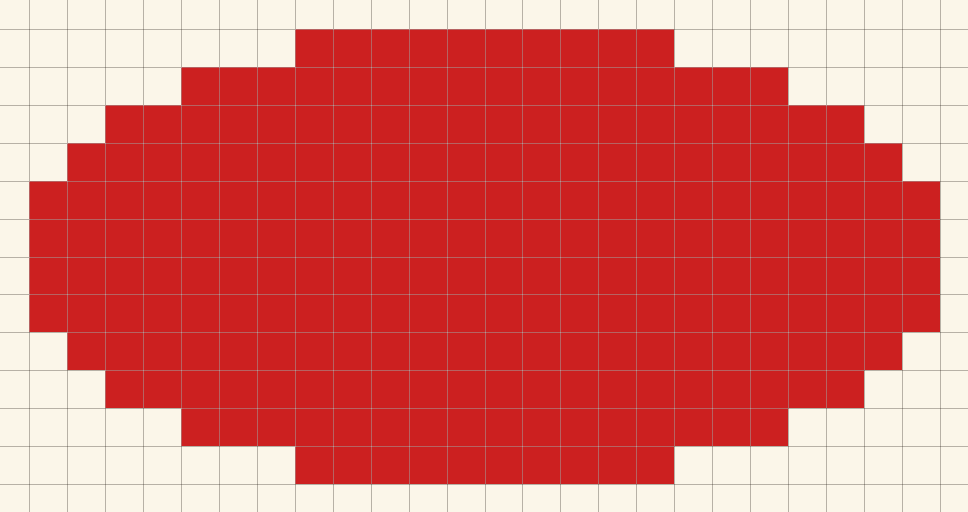
\includegraphics[width=0.5\textwidth]{fig04_2d_ellipse_24x12.png}
\caption{Elipse $W = 24, H = 12$ no Pixel Round. Note como as células ao longo do eixo maior são mais espaçadas que ao longo do eixo menor --- reflexo direto dos semi-eixos diferentes.}
\label{fig:elipse}
\end{figure}

\subsection{Modo 3D e estilos de renderização}

\begin{enumerate}[leftmargin=1.5em,itemsep=0.15em,topsep=0.3em]
  \item Trocar o modo para \acc{3D / Esfera}, tamanho $D = 12$ (cf.\ Figura~\ref{fig:3d-shapes}(a)).
  \item Arrastar com o \emph{mouse} para rotacionar. Aparece uma esfera composta de voxels.
  \item Acionar o \emph{Info chip}: anotar o volume.
  \item Trocar para \acc{Elipsóide}, $W = 20$, $H = 10$, $D = 12$ (cf.\ Figura~\ref{fig:3d-shapes}(b)).
  \item Demonstrar o \emph{slider Cut} no eixo \texttt{Y}, 50\% (ver Figura~\ref{fig:cortes}(a)). Observar a metade superior desaparecer.
  \item Alternar para o eixo diagonal $\swarrow$/$\nearrow$ ($45^\circ$, Figura~\ref{fig:cortes}(c)). Discutir o corte oblíquo.
  \item Testar os três \emph{estilos 3D} (\acc{Clássico}, \acc{Suave}, \acc{Blocos}) --- a Figura~\ref{fig:styles} mostra a diferença.
\end{enumerate}

\begin{figure}[H]
\centering
\begin{subfigure}[t]{0.27\linewidth}\centering
  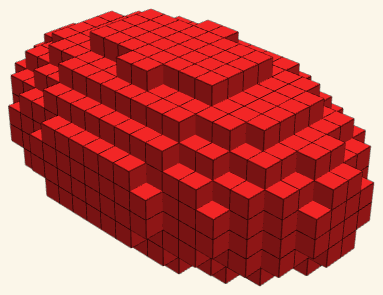
\includegraphics[width=\linewidth]{fig08_3d_ellipsoid.png}
  \caption{\emph{Clássico}}
\end{subfigure}\hfill
\begin{subfigure}[t]{0.27\linewidth}\centering
  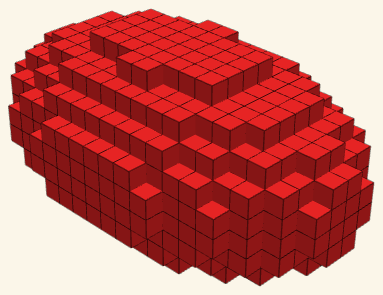
\includegraphics[width=\linewidth]{fig12_3d_style_smooth.png}
  \caption{\emph{Suave}}
\end{subfigure}\hfill
\begin{subfigure}[t]{0.27\linewidth}\centering
  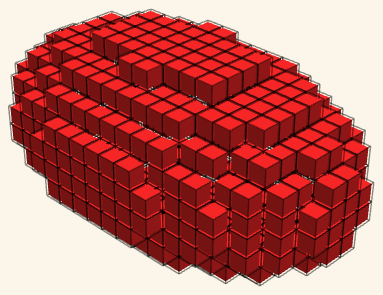
\includegraphics[width=\linewidth]{fig13_3d_style_blocks.png}
  \caption{\emph{Blocos}}
\end{subfigure}
\caption{Três estilos de sombreamento 3D para o mesmo elipsóide. \emph{Clássico} marca bem luz e sombra; \emph{Suave} reduz o contraste para um aspecto mais uniforme; \emph{Blocos} introduz reentrância geométrica nas faces, útil para visualizar a estrutura cúbica.}
\label{fig:styles}
\end{figure}

\subsection{Exportação}
\begin{enumerate}[leftmargin=1.5em,itemsep=0.15em,topsep=0.3em]
  \item Mostrar o botão de \emph{download} no canto do canvas.
  \item Clicar e demonstrar o salvamento como PNG.
  \item Observar: o PNG sai em alta resolução, ideal para imprimir, projetar ou colar em redações multimodais (incluindo as do ENEM).
\end{enumerate}

% =============================================================================
\newpage
\section{Lista de exercícios}\label{ap:exerc}

\textbf{Instruções:} responder individualmente. Pode-se consultar o Pixel Round para confirmar respostas, \emph{mas a justificativa matemática é obrigatória}. Entregar manuscrita ou digitada.

\subsection*{Exercício 1 --- Equação da circunferência}
\textbf{Enunciado:} Considere uma circunferência centrada na origem $(0, 0)$ com raio $r = 7$. Verifique se cada um dos pontos a seguir está \emph{dentro}, \emph{fora} ou \emph{sobre} a circunferência. Justifique com a equação.
\begin{enumerate}[label=\alph*),leftmargin=1.5em,itemsep=0.1em,topsep=0.2em,nosep]
  \item $(3, 4)$ \hfill \emph{gabarito:} dentro ($9 + 16 = 25 < 49$).
  \item $(5, 5)$ \hfill \emph{gabarito:} \acc{fora} ($25 + 25 = 50 > 49$, pois $\sqrt{50} \approx 7{,}07$).
  \item $(0, 7)$ \hfill \emph{gabarito:} sobre.
  \item $(-7, 0)$ \hfill \emph{gabarito:} sobre.
\end{enumerate}

\textit{Atenção pedagógica:} o item (b) é uma armadilha proposital.

\subsection*{Exercício 2 --- Critério euclidiano em uma célula}
\textbf{Enunciado:} Uma circunferência tem centro em $(5, 5)$ e raio $5$. Aplique o critério euclidiano à célula $(i, j) = (1, 3)$: ela é pintada?

\emph{Gabarito:} centro da célula em $(1{,}5,\, 3{,}5)$. Distância ao centro da circunferência: $\sqrt{(5{-}1{,}5)^2 + (5{-}3{,}5)^2} = \sqrt{12{,}25 + 2{,}25} = \sqrt{14{,}5} \approx 3{,}81$. Como $3{,}81 < 5$, a célula é \acc{pintada}.

\subsection*{Exercício 3 --- Área discreta \emph{vs.} contínua}
\textbf{Enunciado:} No Pixel Round, gere um círculo de diâmetro $D = 20$ no algoritmo Euclidiano (cf.\ Figura~\ref{fig:comp-d20}(a)). Anote a área discreta (em pixels). Calcule a área contínua: $\pi r^2$. Calcule o erro relativo. Em seguida, repita para o algoritmo \emph{Limiar} (Figura~\ref{fig:comp-d20}(c)). Compare.

\emph{Gabarito esperado:} a área contínua é $\pi \cdot 100 \approx 314{,}16$. O Euclidiano costuma aproximar com erro abaixo de $2\%$. O \emph{Limiar} costuma sobreestimar em 5--8\%.

\subsection*{Exercício 4 --- Volume do elipsóide e corte (estilo ENEM)}
\textbf{Enunciado:} Considere um elipsóide com semi-eixos $r_x = 4$, $r_y = 6$, $r_z = 3$.
\begin{enumerate}[label=\alph*),leftmargin=1.5em,itemsep=0.1em,topsep=0.2em,nosep]
  \item Calcule o volume contínuo.
  \item Após um corte no eixo $Y$ que preserva $50\%$ da altura (Figura~\ref{fig:cortes}(a)), qual o volume restante (continuamente)?
  \item Descreva matematicamente o corte como uma desigualdade aplicada à coordenada $y$ do voxel.
\end{enumerate}

\emph{Gabarito:}
(a) $V = \tfrac{4}{3}\pi \cdot 4 \cdot 6 \cdot 3 = 96\pi \approx 301{,}59$.
(b) Pela simetria, metade: $\approx 150{,}80$.
(c) $y < \mathit{cut}$, onde $\mathit{cut} = 0{,}5 \cdot D_y = 0{,}5 \cdot 12 = 6$.

\subsection*{Exercício 5 --- Roteiro do projeto final}
\textbf{Enunciado:} Após produzir a imagem autoral em grupo (Atividade~\ref{at:42}), responda:
\begin{enumerate}[label=(\arabic*),leftmargin=1.7em,itemsep=0.15em,topsep=0.2em,nosep]
  \item Liste as figuras geométricas usadas (círculo, elipse, esfera, elipsóide) e seus parâmetros (diâmetro ou semi-eixos).
  \item Para a figura principal, qual algoritmo foi escolhido? Por quê? Que efeito visual ele produz que os outros dois não produziriam? (Compare com as Figuras~\ref{fig:comp-d10} e~\ref{fig:comp-d20}.)
  \item Houve cortes 3D? Se sim, descreva matematicamente \emph{um} deles como desigualdade.
  \item \emph{(Opcional)} Sua produção dialoga com alguma referência cultural brasileira (modernismo, arte concreta, grafismo indígena, arquitetura de Niemeyer)? Comente.
\end{enumerate}

% =============================================================================
\newpage
\section{Adaptação para escolas sem laboratório de informática}\label{ap:adapt-analog}

Esta adaptação possibilita aplicar a sequência \emph{integralmente em papel} quando o acesso a computador estiver inviabilizado --- realidade frequente em escolas do campo, escolas indígenas e quilombolas, em comunidades ribeirinhas da Amazônia, e em escolas estaduais de pequenos municípios. O eixo conceitual permanece intacto; o que muda é o suporte material.

\subsection{Substituições por aula}

\begin{center}
\small
\begin{tabularx}{\textwidth}{@{}p{0.16\textwidth}p{0.36\textwidth}X@{}}
\toprule
\textbf{Aula} & \textbf{Atividade original} & \textbf{Adaptação analógica} \\
\midrule
1 & Demonstração do Pixel Round (1.3) & Professor desenha à mão três versões da circunferência $D = 10$ em uma malha pré-impressa do tamanho da lousa --- uma por algoritmo. As Figuras~\ref{fig:comp-d10} e~\ref{fig:comp-d20} deste plano podem ser impressas como referência. \\
\addlinespace[3pt]
2 & Comparação quantitativa no software (\ref{at:25}) & Distribuir folhas com as três circunferências de $D = 16$ pré-desenhadas (impressas das Figuras deste plano) e pedir a contagem manual. \\
\addlinespace[3pt]
3 & Geração da esfera 3D (\ref{at:31},~\ref{at:32}) & Distribuir folhas com \emph{fatias} da esfera ($z = 0, 1, 2, \ldots$) em papel quadriculado. O estudante constrói o modelo mental por empilhamento. \\
\addlinespace[3pt]
4 & Produção no Pixel Round (\ref{at:42}) & Produção \emph{exclusivamente} em papel quadriculado com lápis de cor. A defesa matemática (\ref{at:43}) permanece idêntica. \\
\bottomrule
\end{tabularx}
\end{center}

\subsection{Folhas auxiliares}
Para a versão analógica completa, recomenda-se preparar previamente:
\begin{itemize}[leftmargin=1.3em,itemsep=0.1em,topsep=0.2em,nosep]
  \item 1 folha A3 com malha $30 \times 30$ desenhada com régua, para uso na lousa magnética ou afixada na parede.
  \item 1 conjunto por estudante de 4 folhas A4 quadriculadas (5\,mm) --- itens consumíveis previstos no kit escolar do PDDE.
  \item 1 folha com as três circunferências comparativas pré-impressas: as Figuras~\ref{fig:comp-d10} (D=10) e~\ref{fig:comp-d20} (D=20) deste plano, em A4, servem como referência.
\end{itemize}

\subsection{Aproveitamento de saberes locais}
Em escolas indígenas ou em comunidades com forte tradição artesanal (renda de bilro em Aracati/CE, cerâmica em Pirenópolis/GO, tecelagem caiçara no litoral norte de SP), a Aula~\ref{aula3} pode ser \emph{enriquecida com uma visita de portadores de saber tradicional}: rendeiras, tecelãs, ceramistas, mostrando como rasterizam círculos em suas linguagens próprias. Essa aproximação realiza o princípio etnomatemático e a \href{https://www.planalto.gov.br/ccivil_03/_ato2007-2010/2008/lei/l11645.htm}{Lei 11.645/2008}.

\textit{Observação geral:} a versão analógica preserva 100\% dos objetivos conceituais; apenas a fluência operacional (\emph{exportar PNG}, \emph{alternar algoritmos com um clique}) é trabalhada de modo limitado. Caso a escola venha posteriormente a obter acesso ao laboratório, uma \emph{aula de complementação} de 30 minutos é suficiente.

% =============================================================================
\newpage
\section{Glossário técnico para o professor}\label{ap:glos}

\begin{itemize}[leftmargin=1.4em,itemsep=0.3em,topsep=0.3em]
  \item \acc{Algoritmo} --- sequência finita e bem definida de instruções para resolver um problema. Os três algoritmos do Pixel Round (cf.\ Figura~\ref{fig:comp-d10}) são procedimentos distintos para o mesmo problema.
  \item \acc{Bresenham (algoritmo de)} --- algoritmo publicado em 1965 por Jack Bresenham (IBM), originalmente para reta, depois estendido por outros autores (Pitteway, Kappel) para elipse. Sua marca é usar \emph{apenas inteiros}. Veja Atividade~\ref{at:23}.
  \item \acc{BNCC} --- Base Nacional Comum Curricular. Documento normativo brasileiro de referência para a Educação Básica, aprovado em 2017 (EI/EF) e 2018 (EM).
  \item \acc{Canvas} --- elemento HTML que disponibiliza um espaço de desenho 2D ou 3D no navegador. Pixel-by-pixel ou via WebGL.
  \item \acc{ENEM} --- Exame Nacional do Ensino Médio. Maior avaliação educacional do Brasil, com participação anual de milhões de estudantes. Articulação detalhada em §\ref{sec:enem}.
  \item \acc{Equação implícita} --- equação da forma $F(x, y) = 0$, em que a curva é definida pelo \emph{zero} da função. A da elipse: $(x/r_x)^2 + (y/r_y)^2 - 1 = 0$.
  \item \acc{Etnomatemática} --- campo de estudos fundado pelo brasileiro Ubiratan D'Ambrosio. Ver §\ref{sec:obmep} e Atividade~\ref{at:34}.
  \item \acc{IMPA} --- Instituto de Matemática Pura e Aplicada (\url{https://impa.br}). Centro de pesquisa de referência mundial sediado no Rio de Janeiro. Organizador da \hyperref[sec:obmep]{OBMEP}.
  \item \acc{LGPD} --- Lei Geral de Proteção de Dados Pessoais (\href{https://www.planalto.gov.br/ccivil_03/_ato2015-2018/2018/lei/l13709.htm}{Lei 13.709/2018}).
  \item \acc{OBMEP} --- Olimpíada Brasileira de Matemática das Escolas Públicas (\url{https://www.obmep.org.br}). Maior olimpíada de matemática do mundo. Detalhes em §\ref{sec:obmep}.
  \item \acc{Pixel} --- abreviação de \emph{picture element}. Unidade mínima de uma imagem digital. Em uma malha, ocupa uma célula $1 \times 1$.
  \item \acc{PWA} --- \emph{Progressive Web App}. Aplicação \emph{web} instalável e operável \emph{offline}.
  \item \acc{Rasterização} --- processo de converter uma descrição geométrica contínua em uma matriz de pixels (no caso 2D) ou voxels (no caso 3D).
  \item \acc{Semi-eixo} --- em uma elipse de centro $C$, é a distância do centro à extremidade da elipse na direção do eixo correspondente. A circunferência é o caso particular em que $r_x = r_y = r$.
  \item \acc{Temperamento igual de 12 tons} --- divisão da oitava em 12 intervalos iguais (semitons), de modo que a razão de frequências entre dois semitons sucessivos é $\sqrt[12]{2} \approx 1{,}0595$. É a base do sistema musical ocidental moderno --- inclusive do samba, do choro e da MPB tradicional.
  \item \acc{Voxel} --- abreviação de \emph{volume element}. Generalização do pixel para 3D: célula cúbica $1 \times 1 \times 1$ em uma malha tridimensional (Figura~\ref{fig:3d-shapes}).
  \item \acc{WebGL} --- biblioteca de programação gráfica em 3D para navegadores. Usada pelo Pixel Round (via \emph{three.js}) para renderizar a cena 3D.
\end{itemize}

\vspace{2em}
\begin{center}
\color{muted}\small\sffamily
--- fim do plano de aula ---
\end{center}

\end{document}
